\documentclass{article}
\usepackage{ucs} 
\usepackage[utf8x]{inputenc} % Включаем поддержку UTF8  
\usepackage{amsmath,amssymb}
\usepackage{tikz}
\usepackage{setspace}
\usepackage{amsfonts}
\usepackage{geometry}
\usepackage{quoting}
\usepackage[russian]{babel}  % Включаем пакет для поддержки русского языка  

\begin{document}
\setlength{\parindent}{0pt}
\begin{Large}
    \textsf{\textbf{ЛинАл ДЗ №6}}
    
    Шамаев Александр    
\end{Large}
\vspace{1cm}

\textsf{\textbf{(1)}}
\begin{quote}
\begin{enumerate}
    \item $\varphi (f_0(x) + f_1(x)) = \begin{pmatrix} f_0(0) + f_1(0) \\ f_0(1) + f_1(1) \end{pmatrix} = \begin{pmatrix} f_0(0) \\ f_0(1) \end{pmatrix} + \begin{pmatrix} f_1(0) \\ f_1(1) \end{pmatrix} = \varphi(f_0(x)) + \varphi(f_1(x))$
    
    \item $\varphi (\alpha f(x)) = \begin{pmatrix} \alpha f(0) \\ \alpha f(1) \end{pmatrix} = \alpha \begin{pmatrix} f(0) \\ f(1) \end{pmatrix} = \alpha \varphi(f(x))$

    $(1)(2) \Longleftrightarrow \varphi$ - ЛО

\end{enumerate}
    \boxed{\text{Ответ: да}}
\end{quote}


\textsf{\textbf{(2)}}
\begin{quote}
    (a)
    
    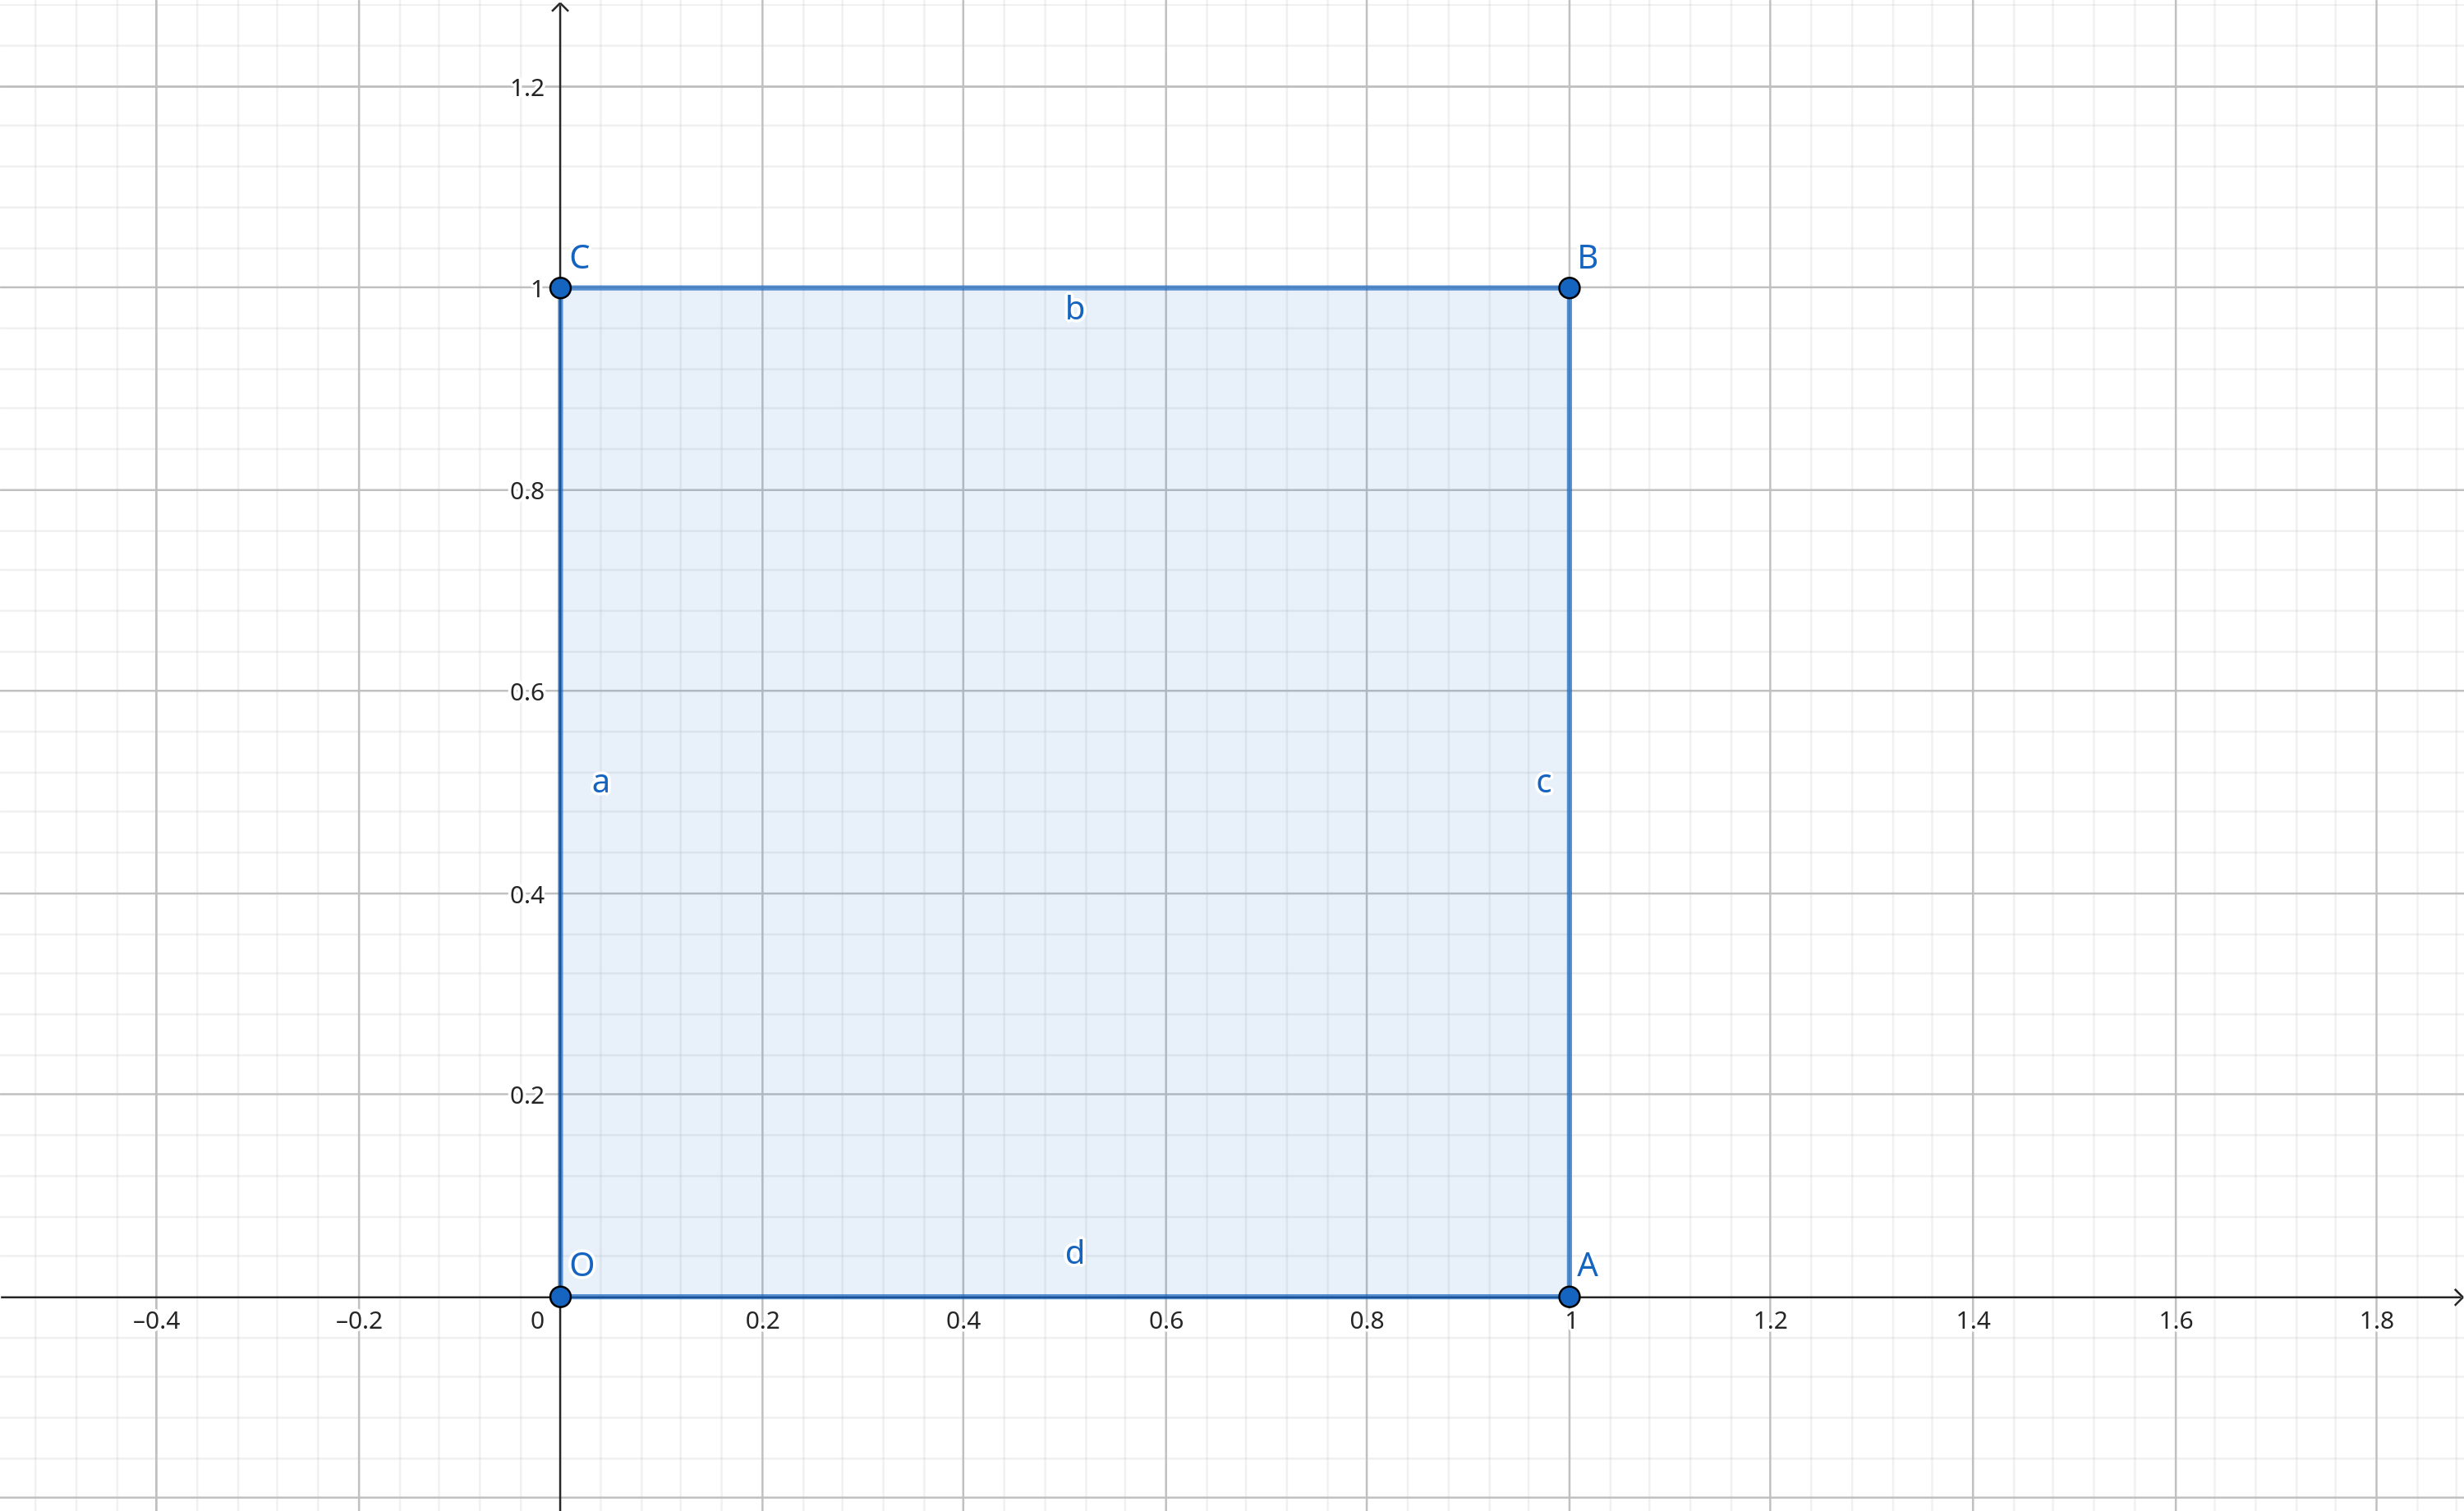
\includegraphics[width=0.70\linewidth]{geogebra-export.png}

    (b)

    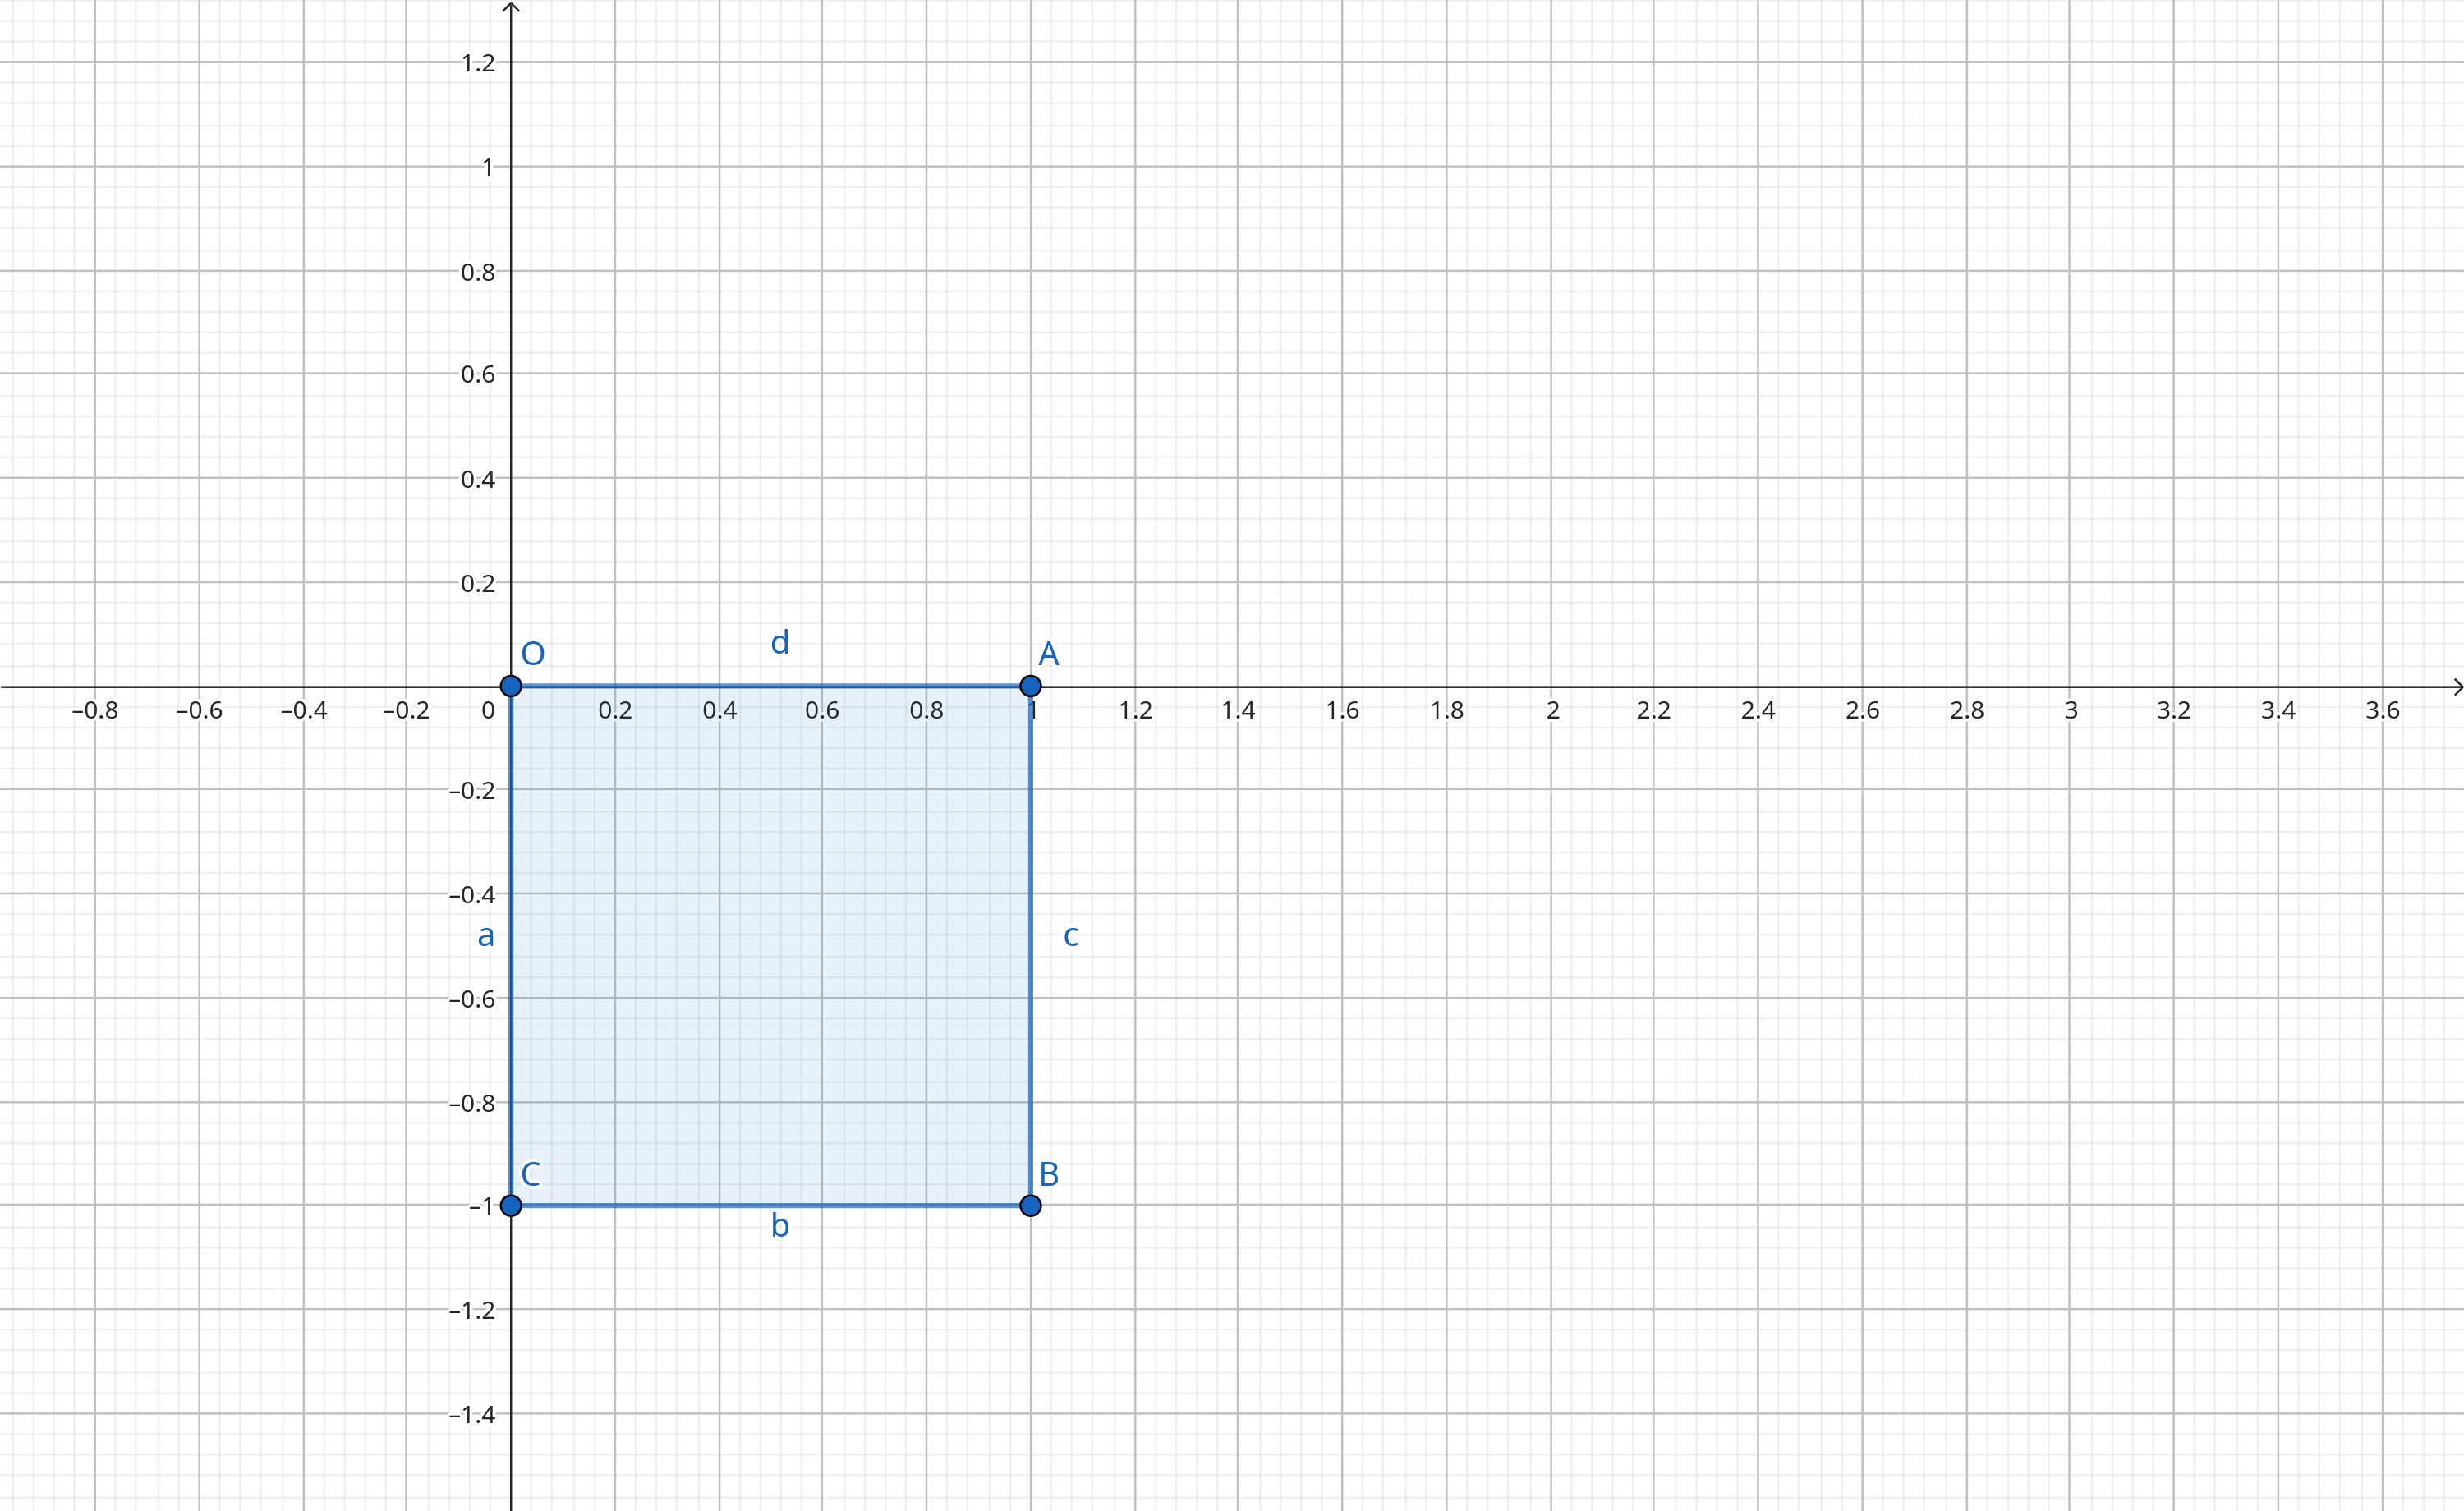
\includegraphics[width=0.70\linewidth]{geogebra-export(1).png}

    (c)

    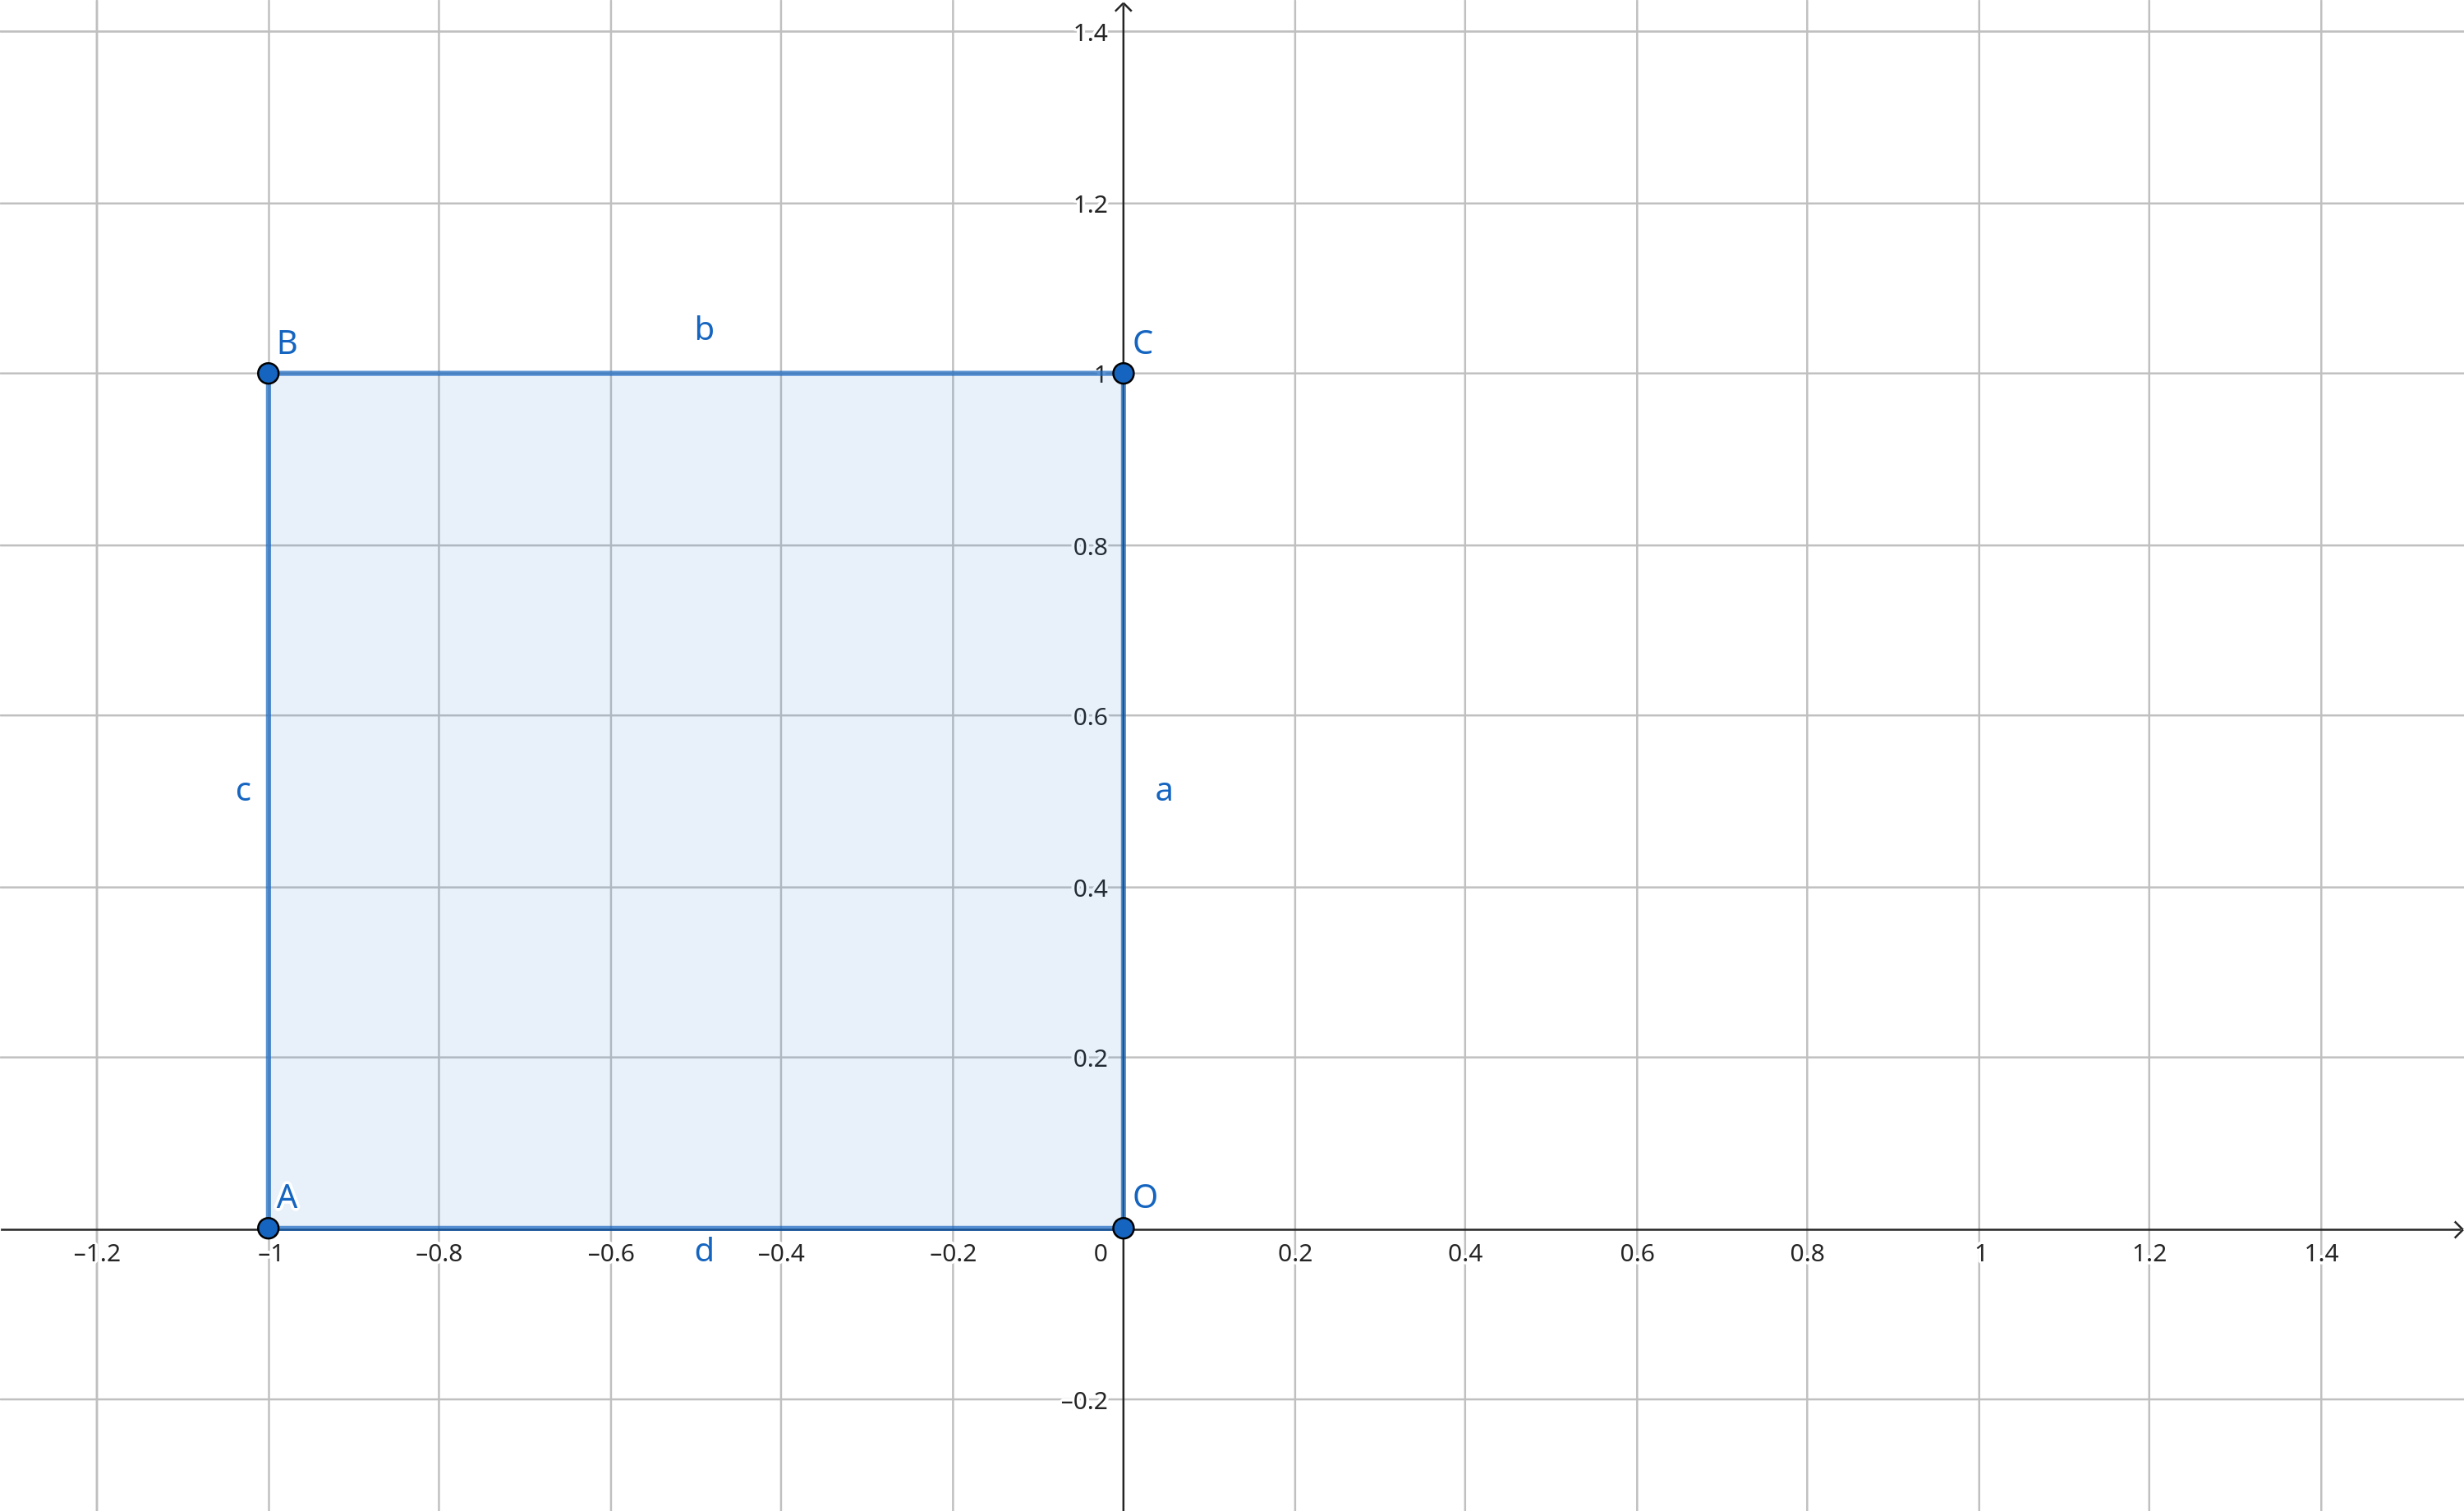
\includegraphics[width=0.75\linewidth]{geogebra-export(2).png}

    (d)

    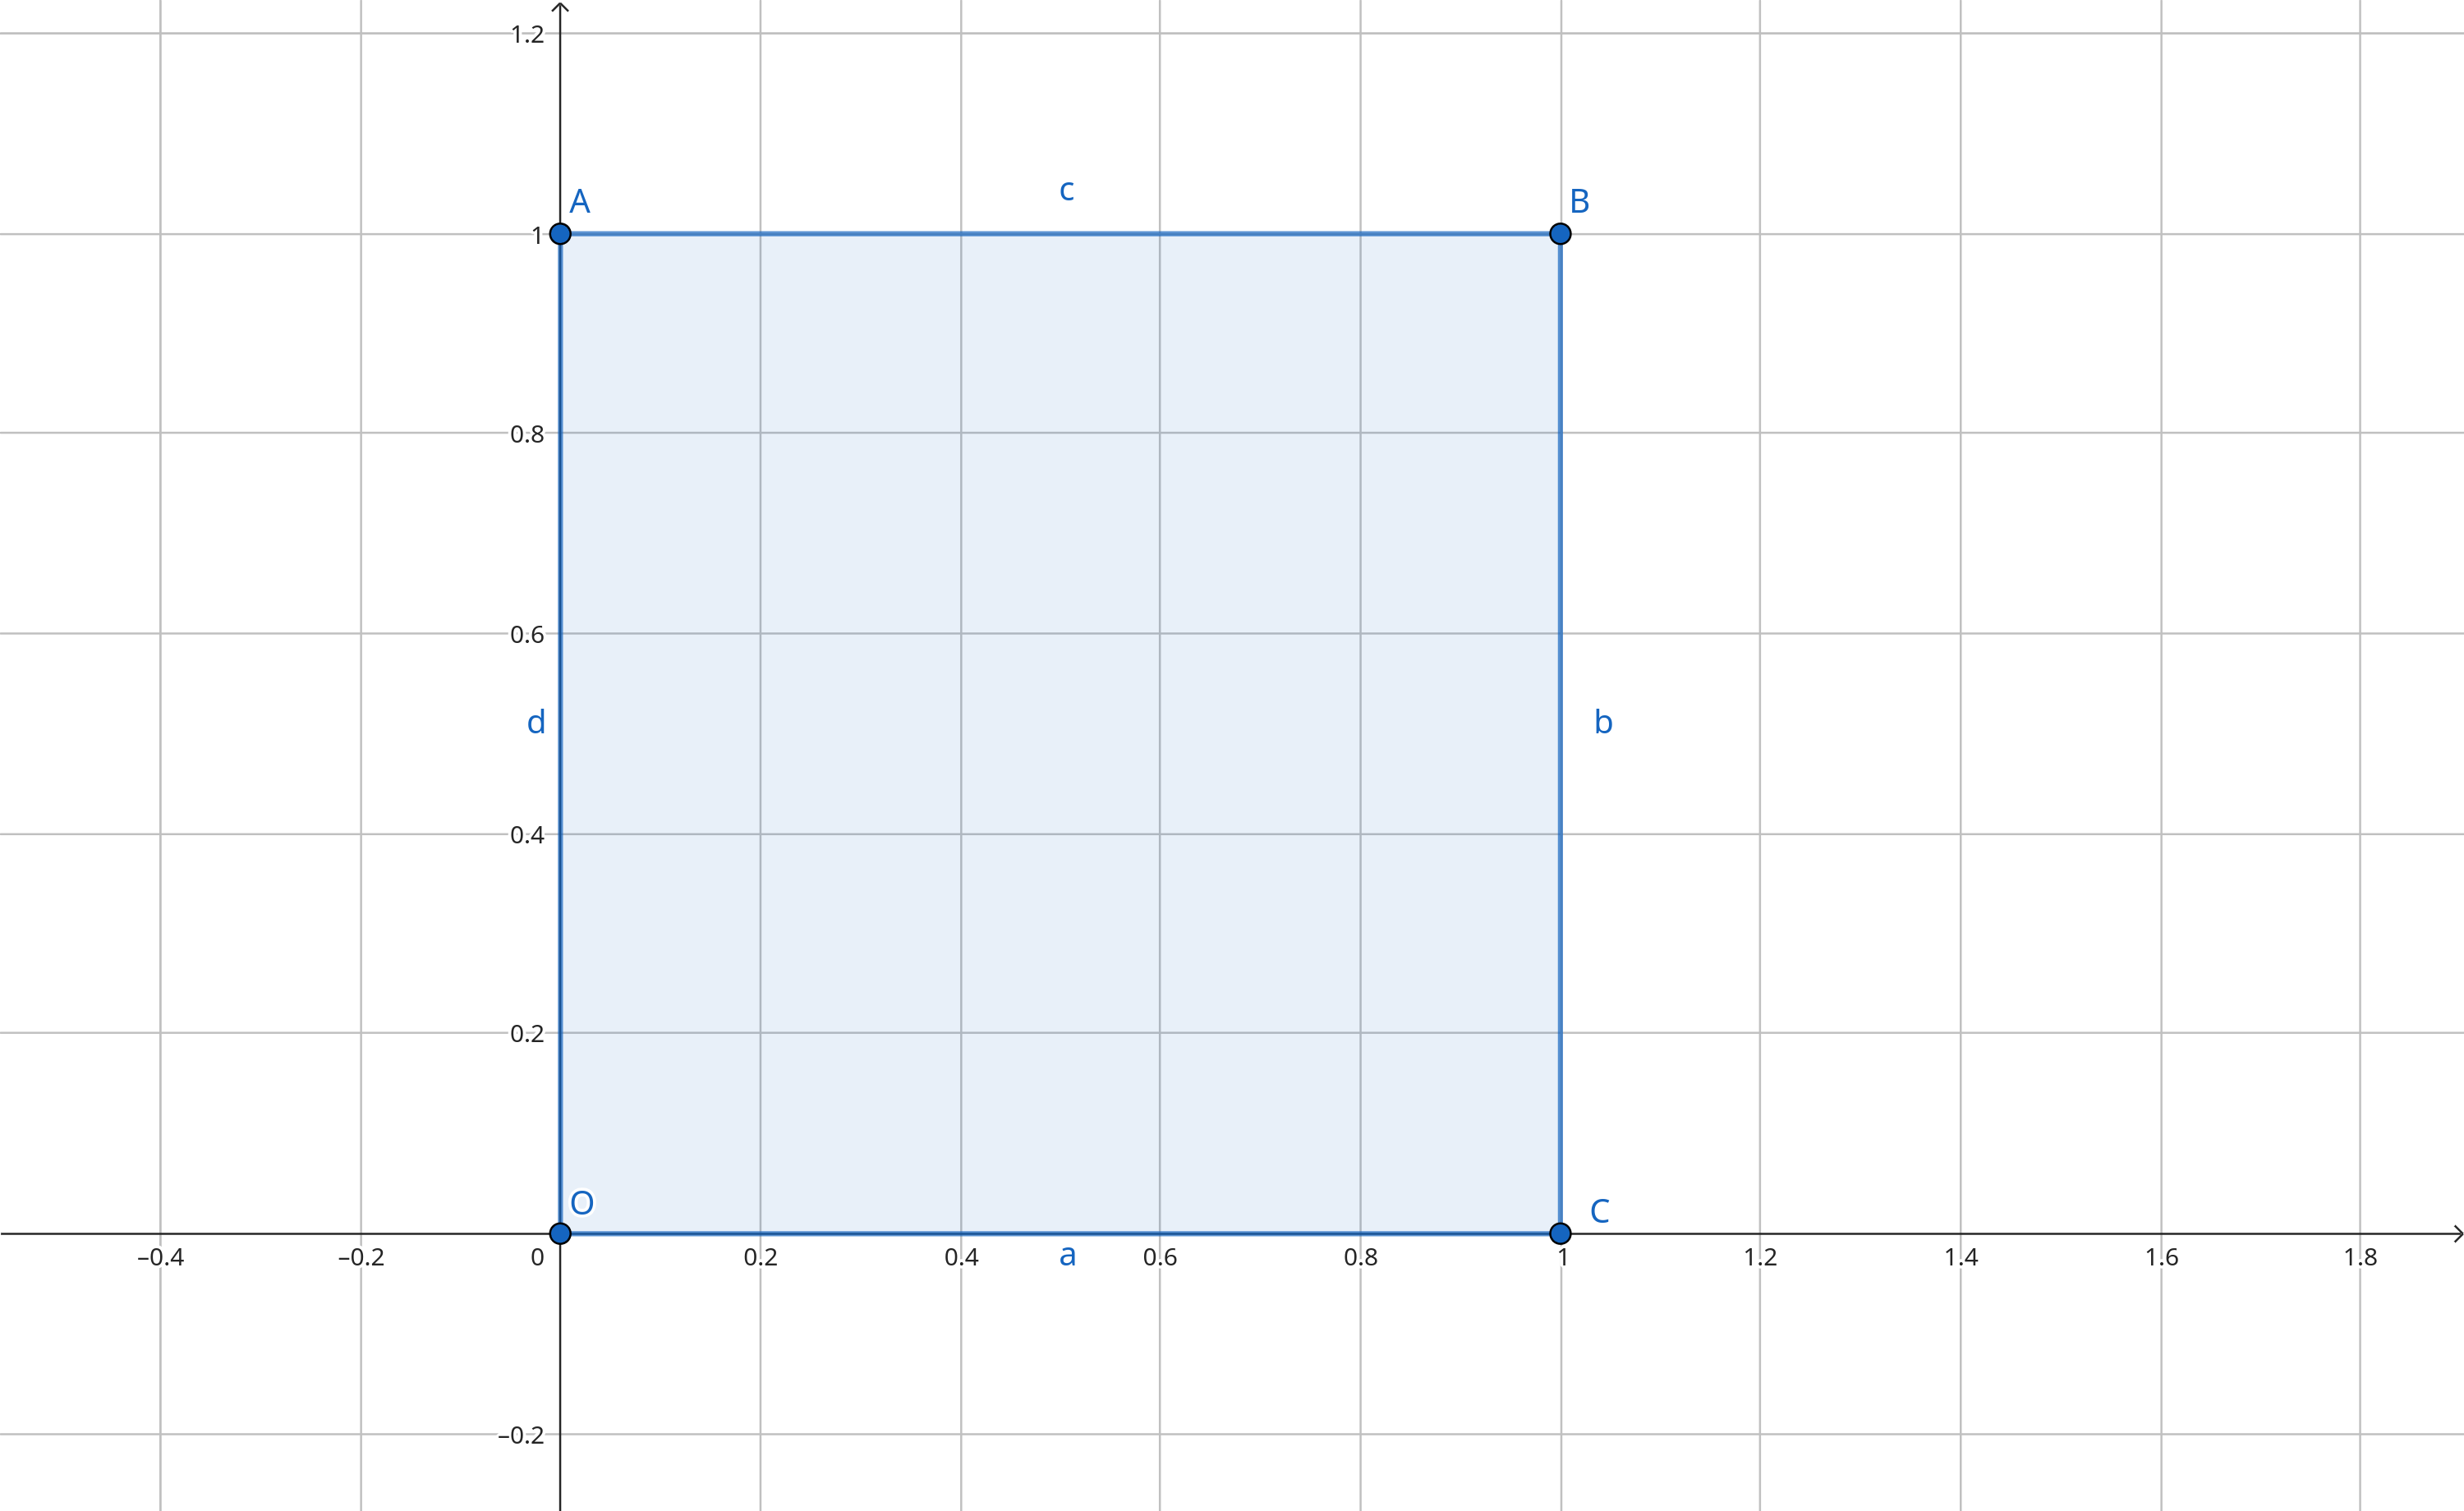
\includegraphics[width=0.75\linewidth]{geogebra-export(3).png}

    (e)
    
    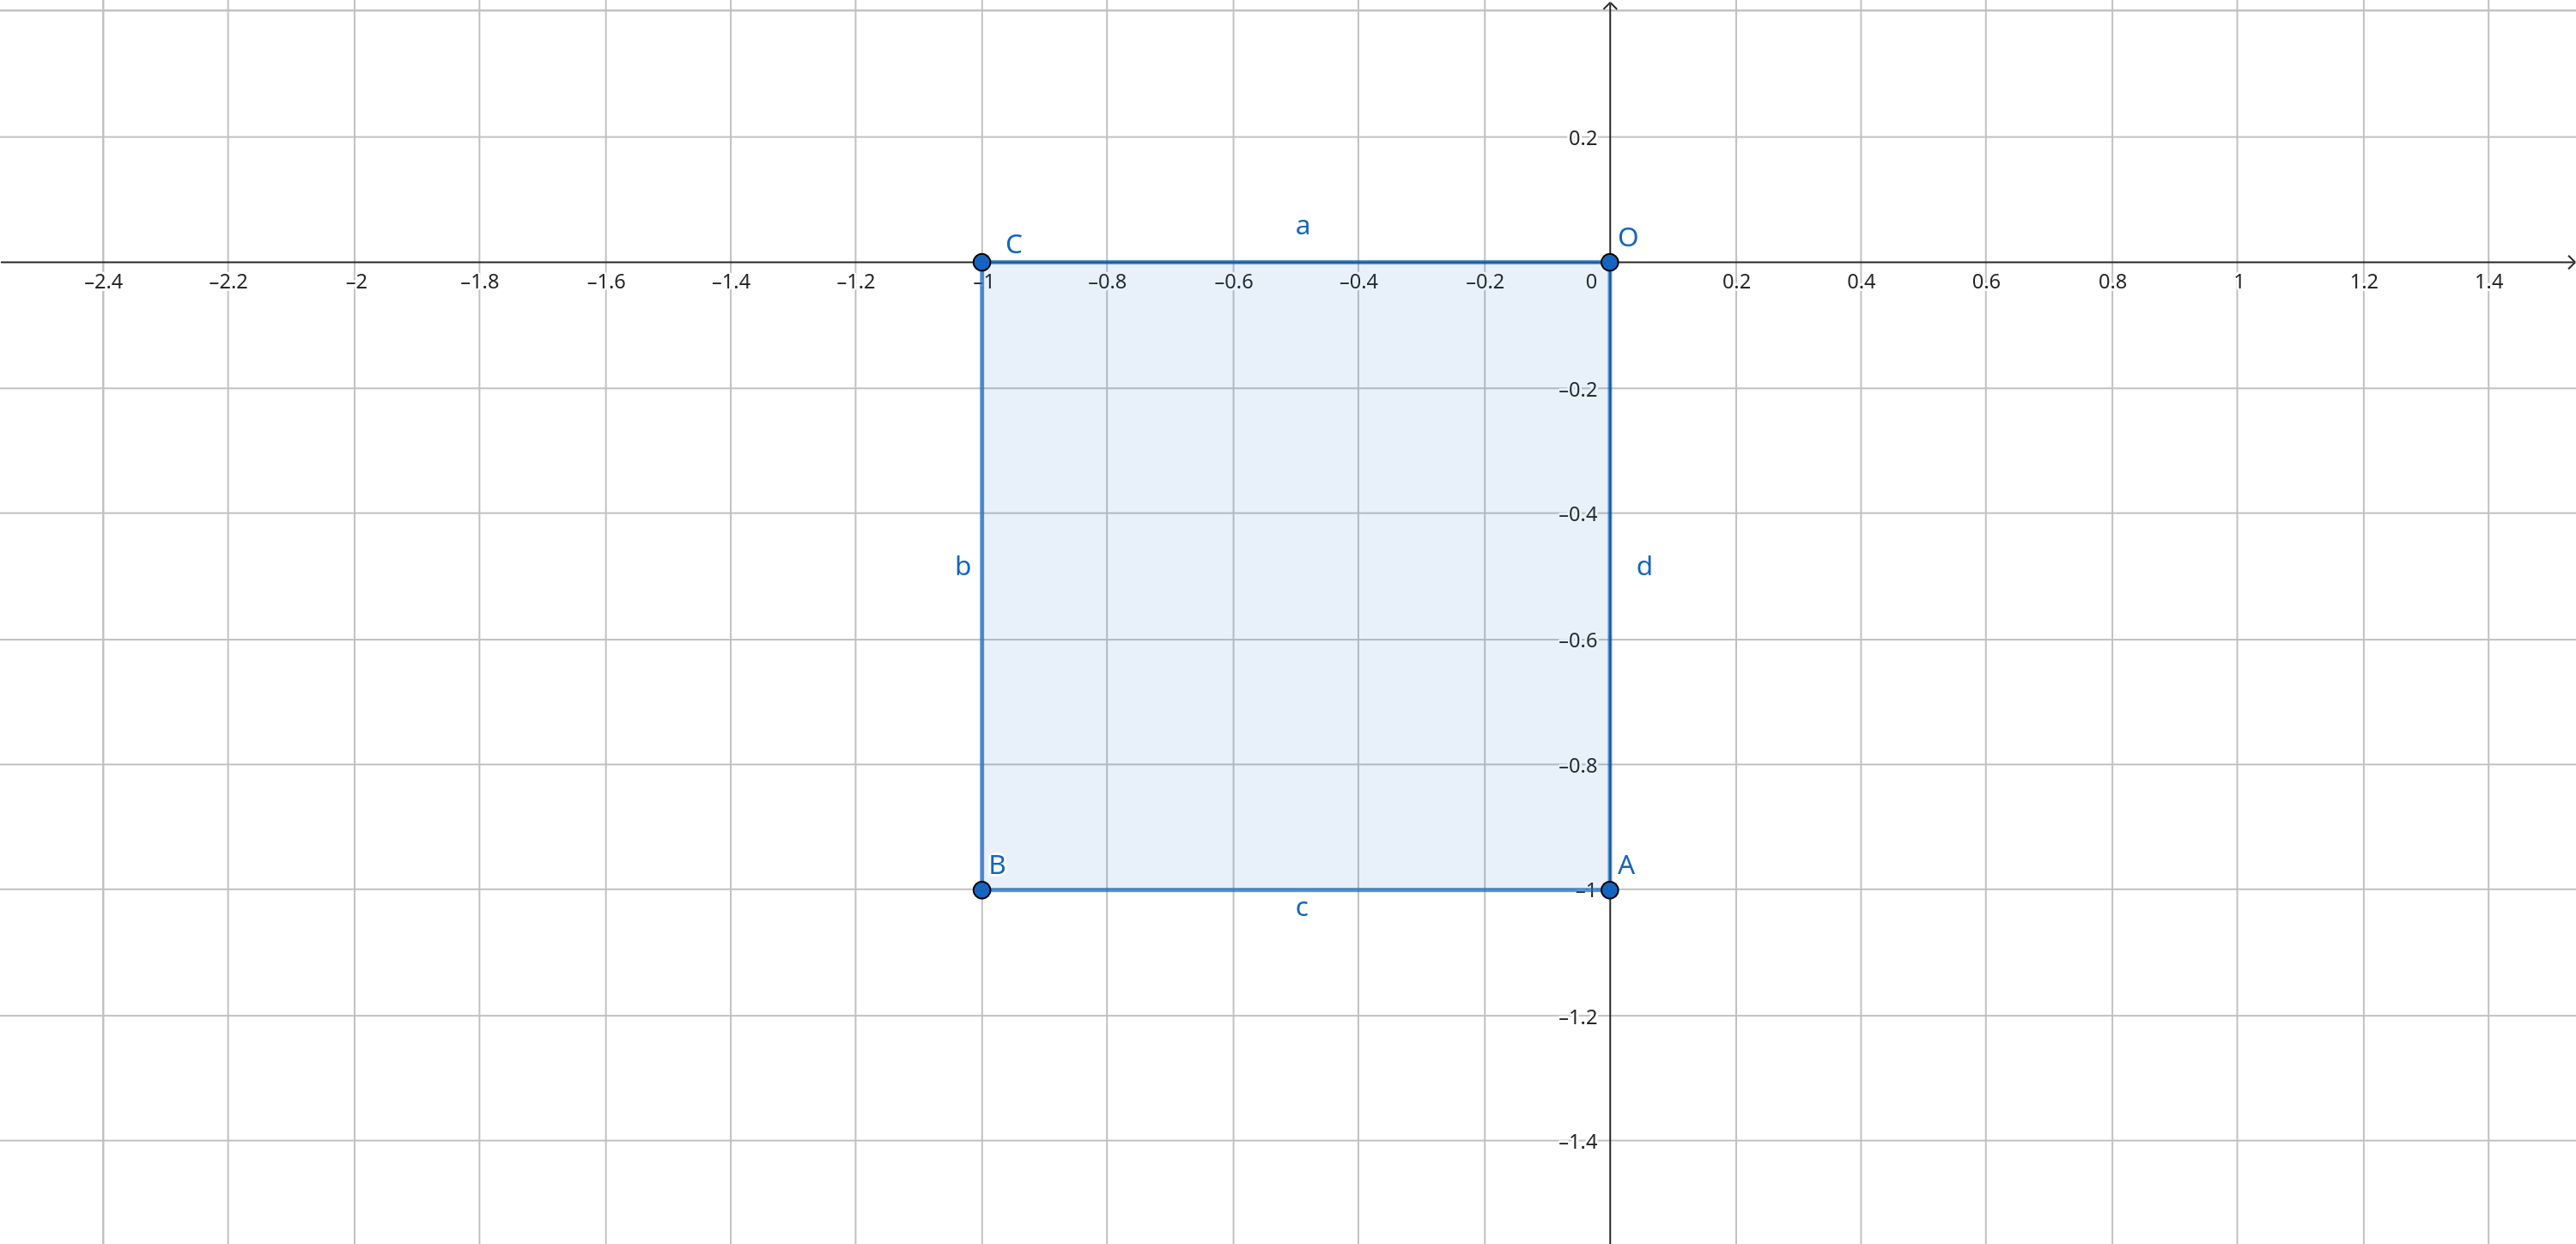
\includegraphics[width=0.75\linewidth]{geogebra-export(4).png}

    (f)

    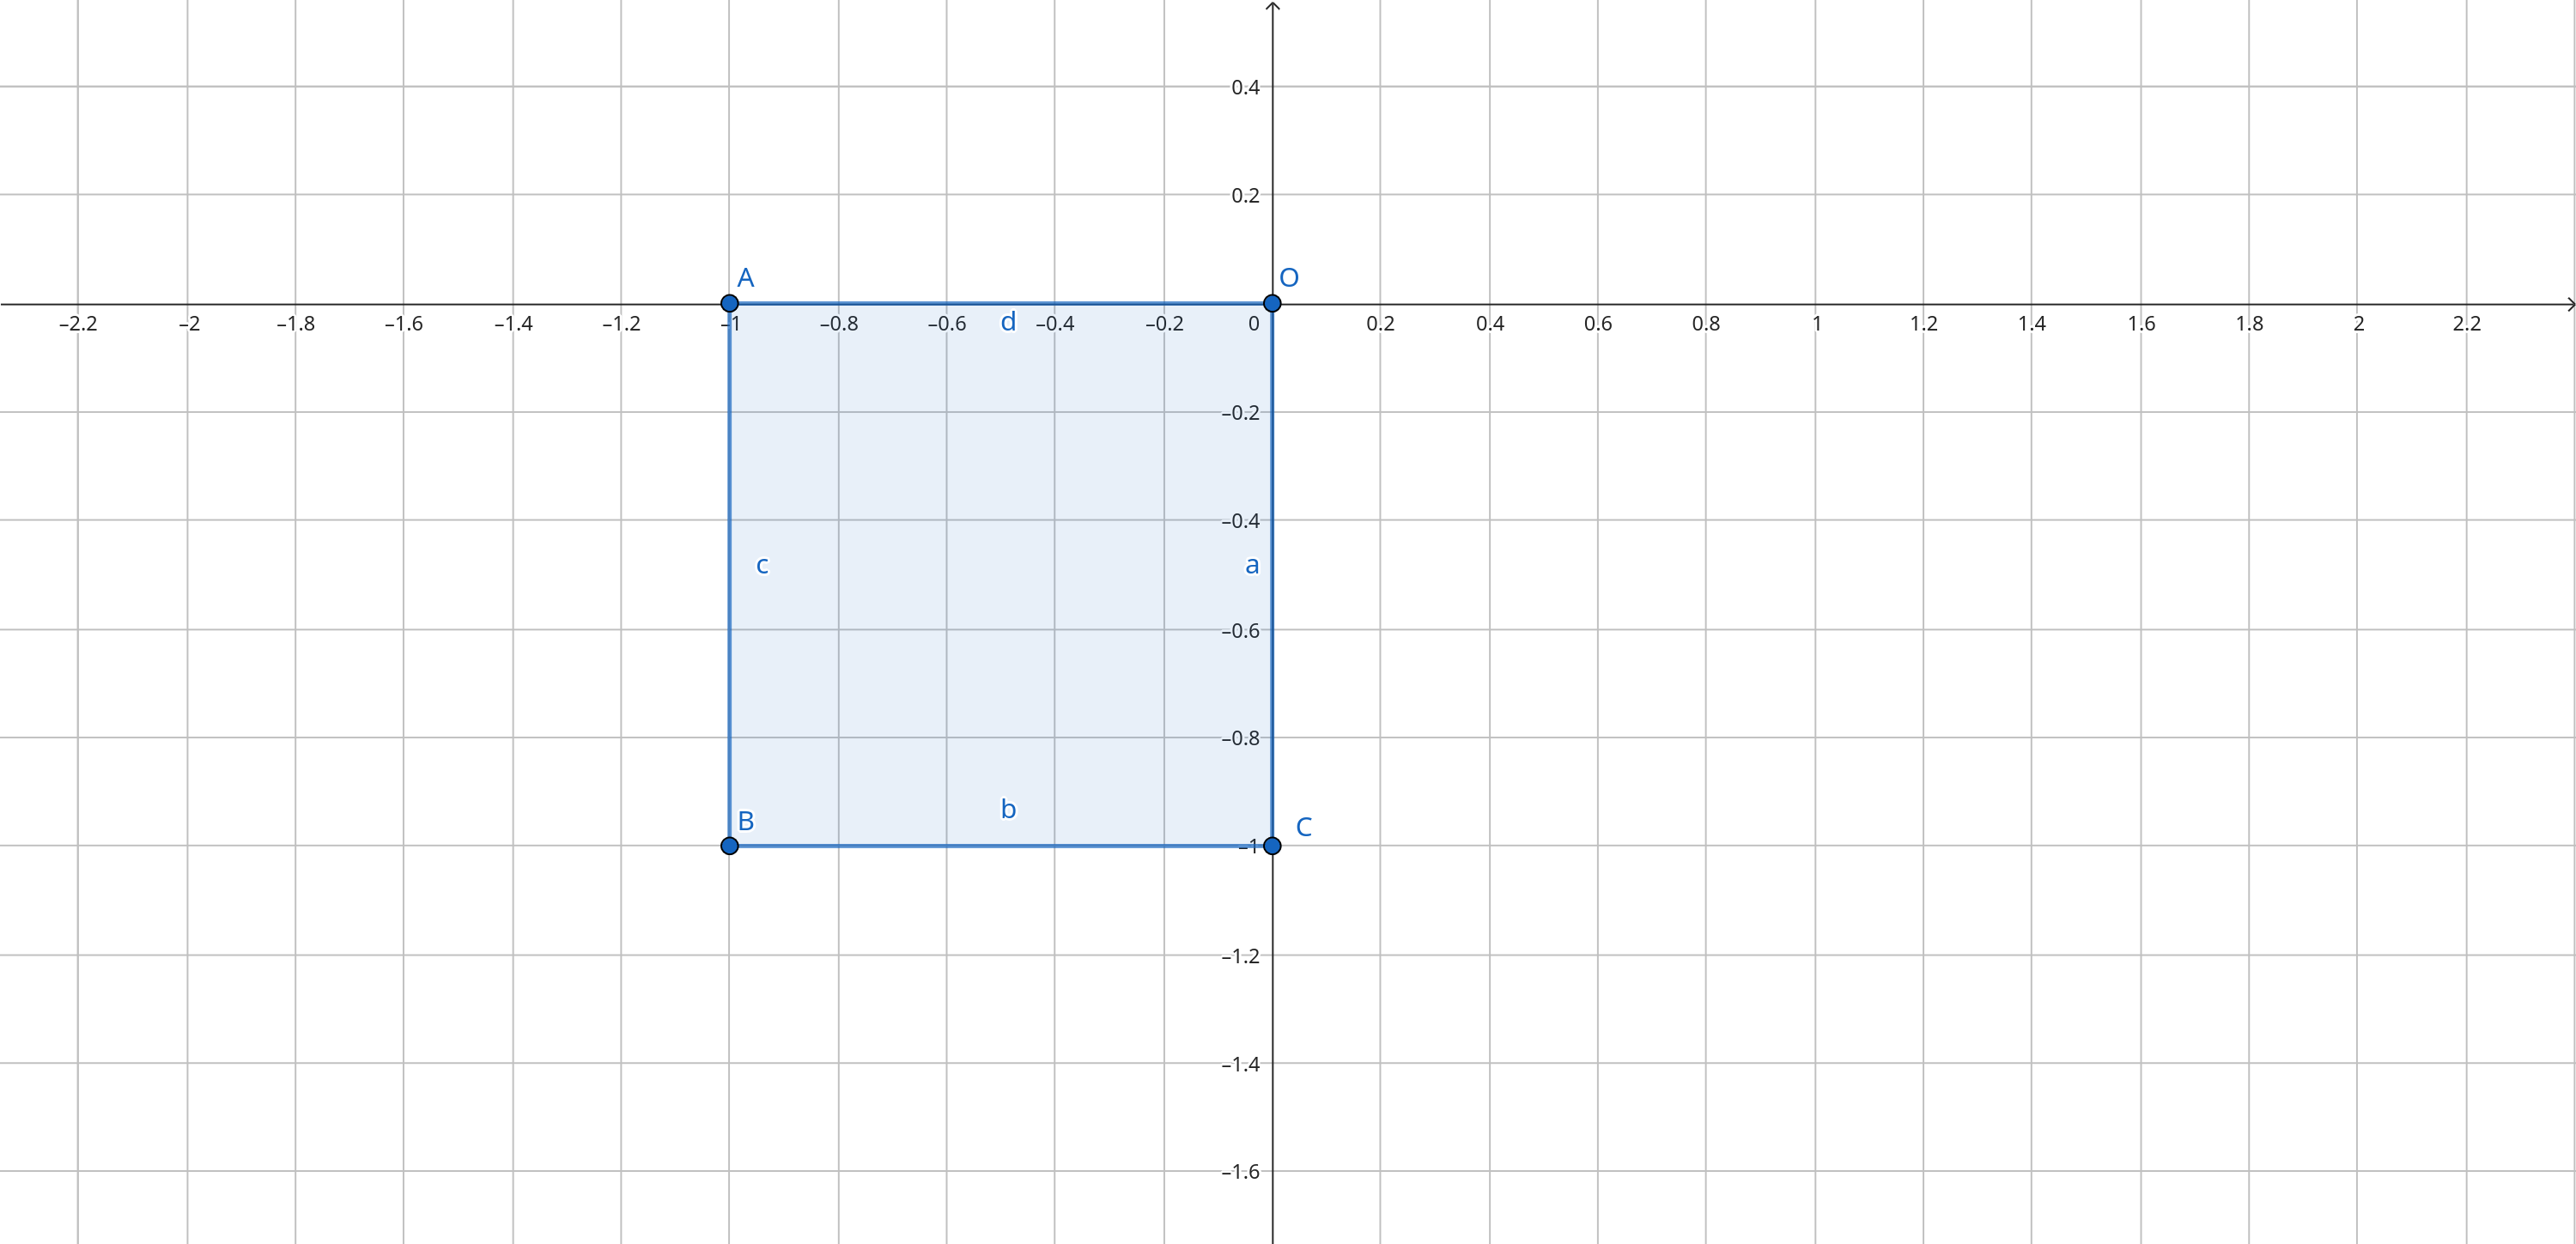
\includegraphics[width=0.75\linewidth]{geogebra-export(5).png}

    (g)

    $A = (k, 0)^T, \ B = (k, 1)^T$
    
    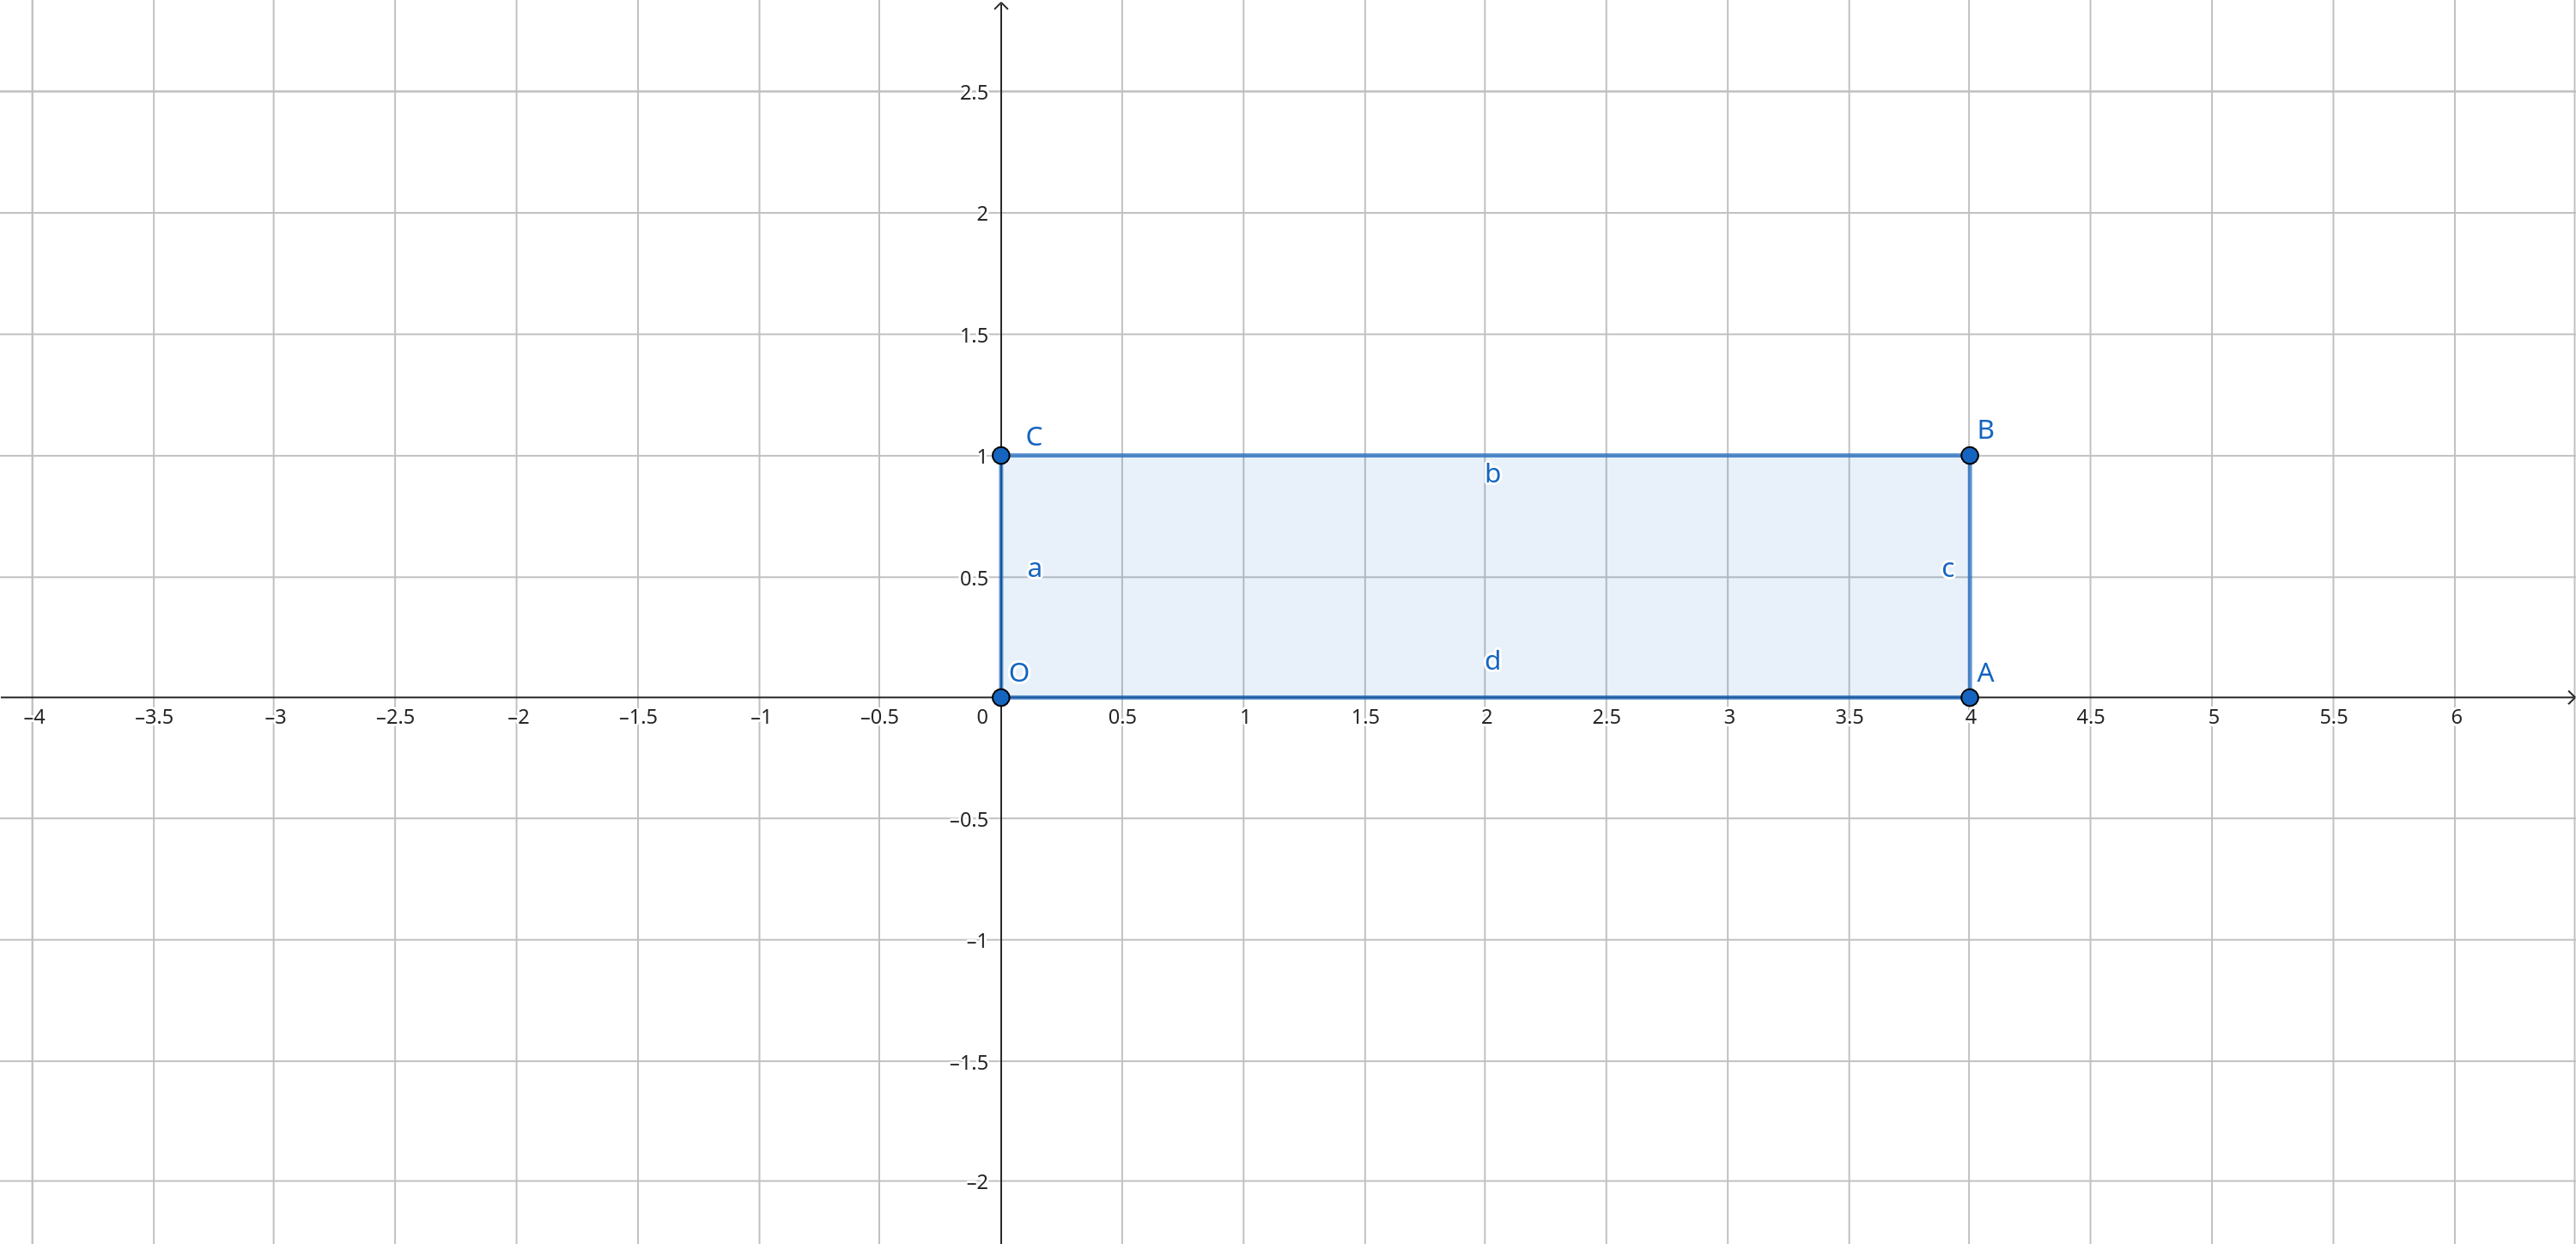
\includegraphics[width=0.75\linewidth]{geogebra-export(6).png}

    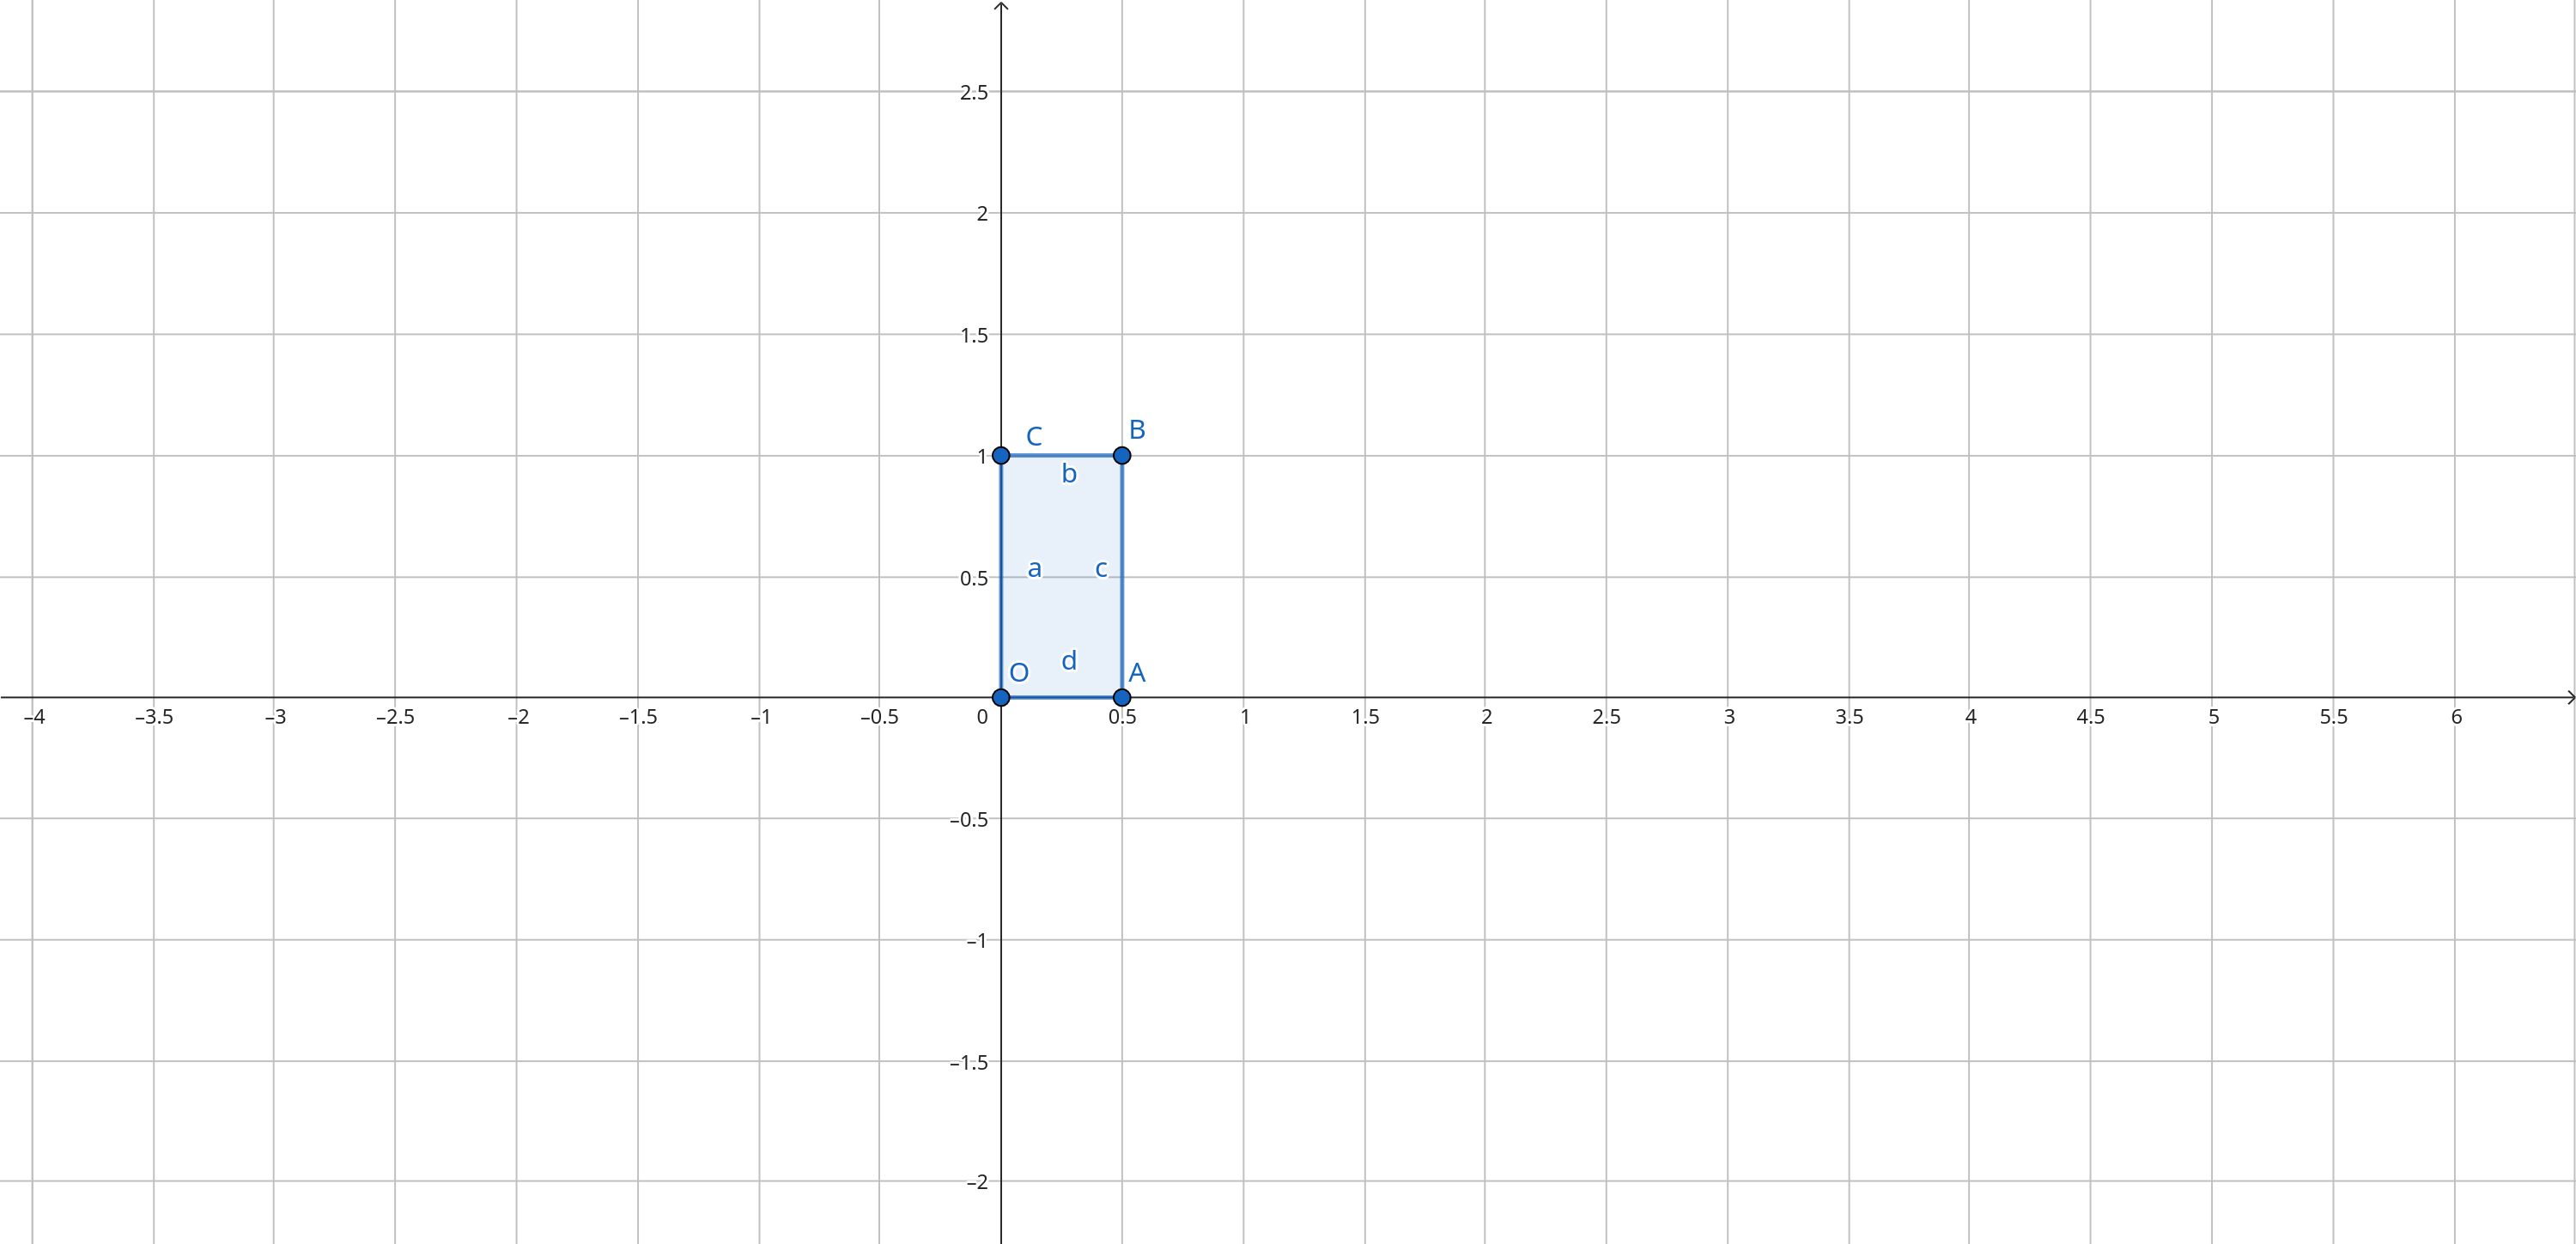
\includegraphics[width=0.75\linewidth]{geogebra-export(7).png}

    (h)
    
    $C = (0, k)^T, \ B = (1, k)^T$
    
        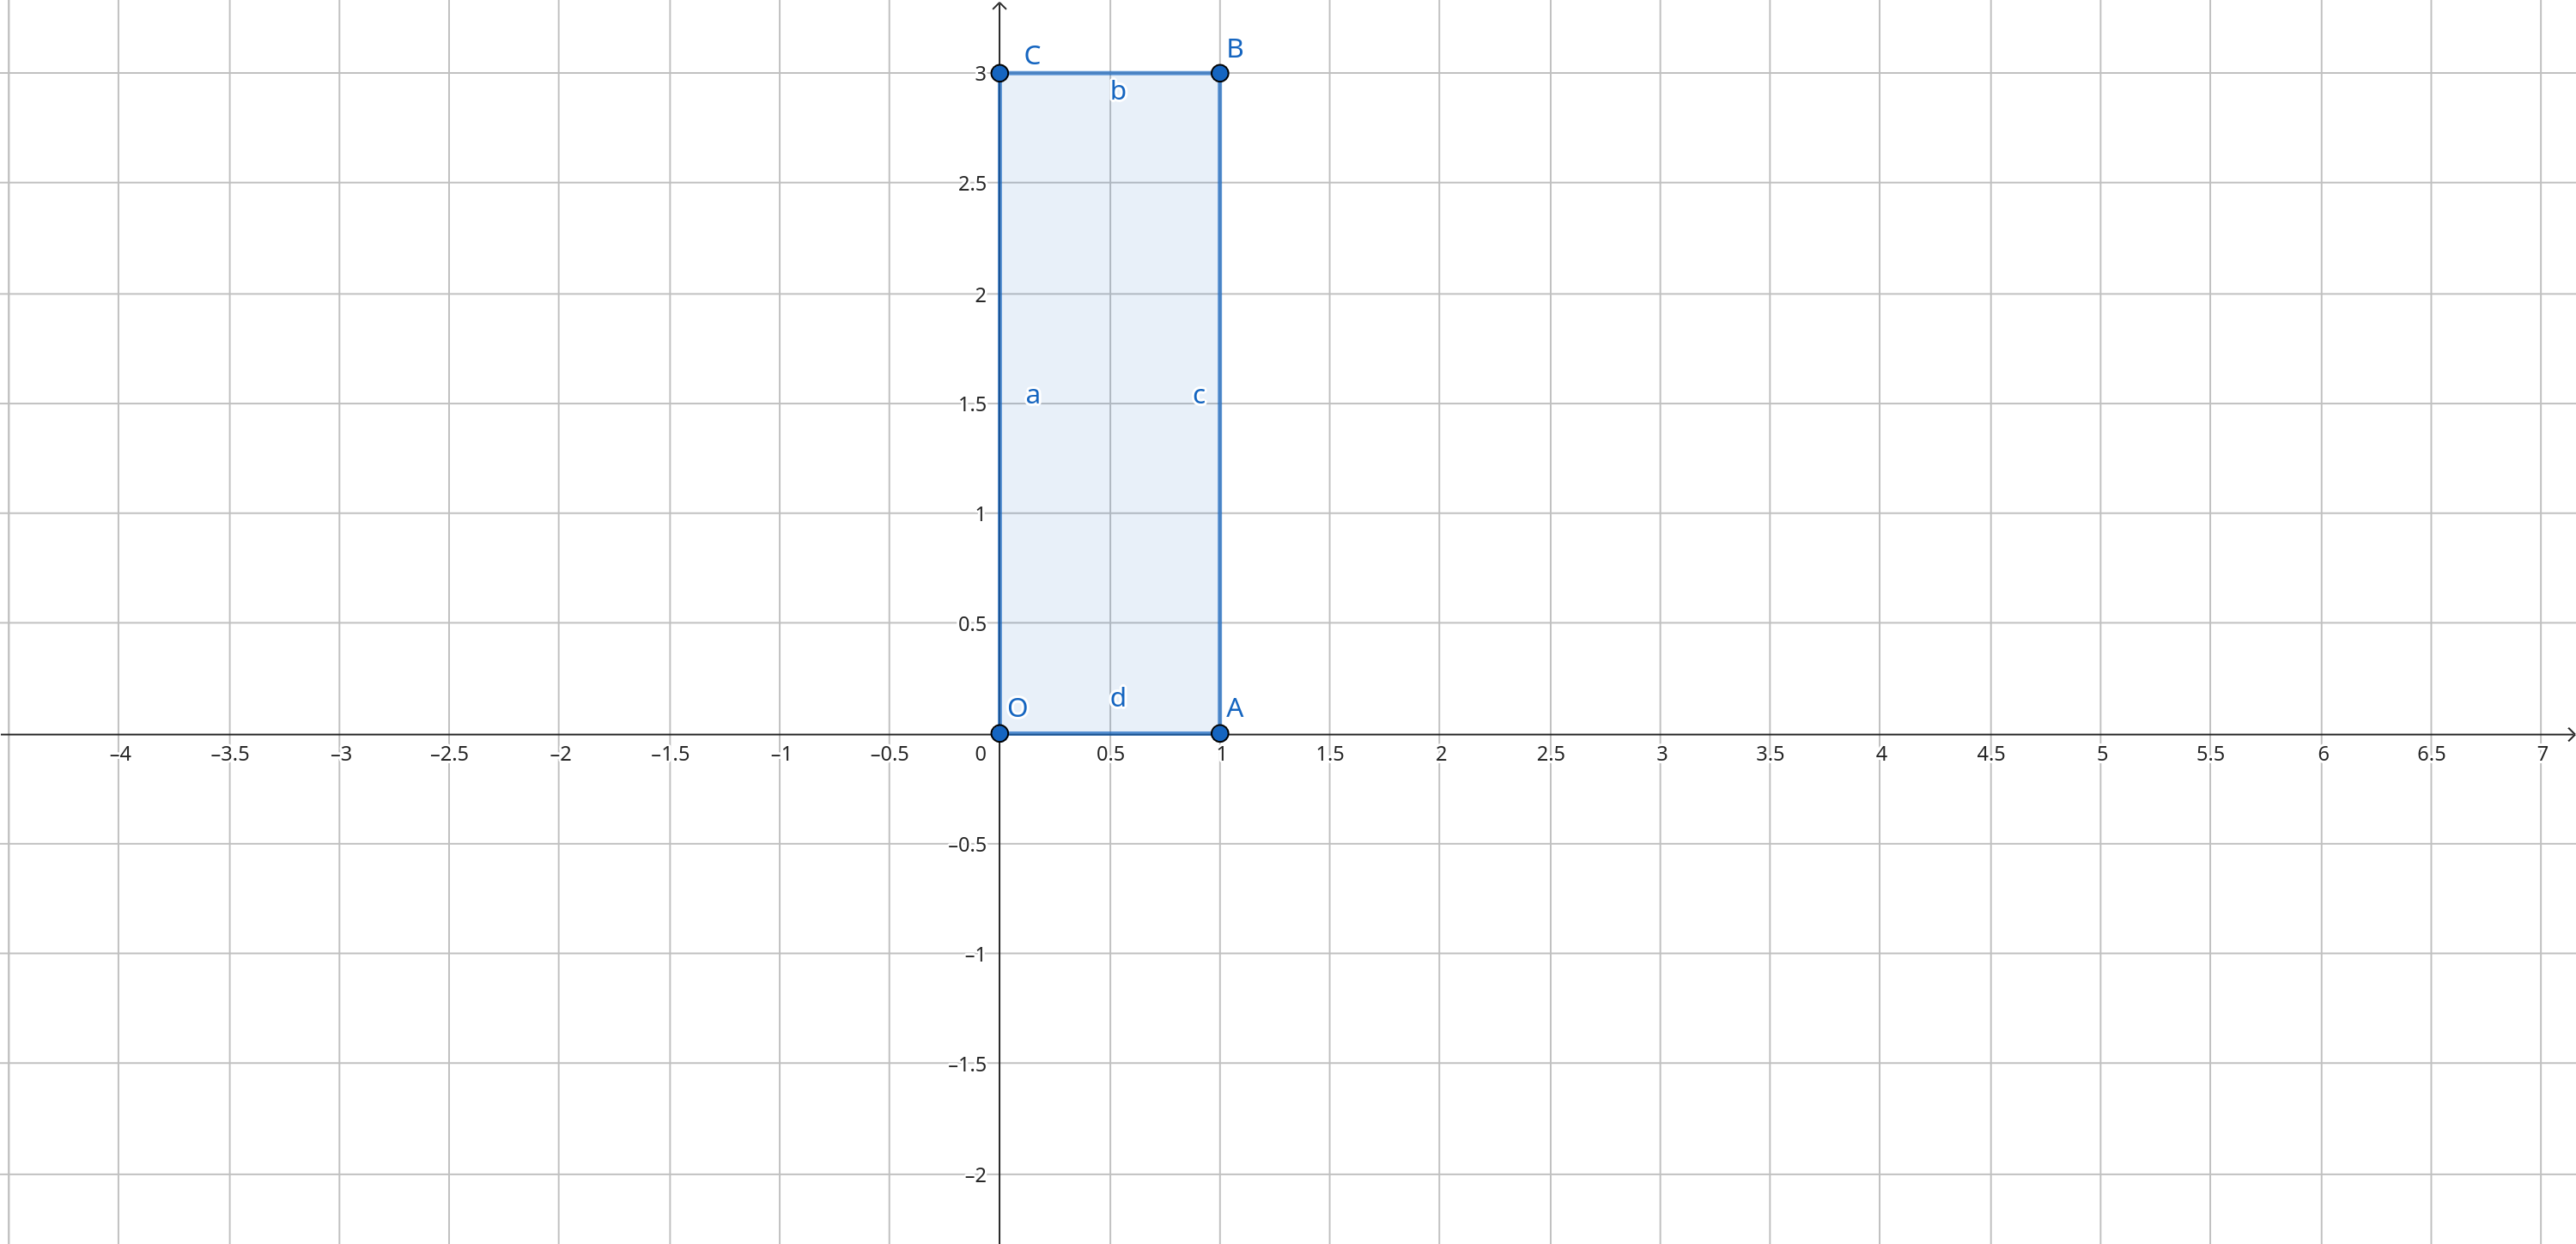
\includegraphics[width=0.75\linewidth]{geogebra-export(8).png}

            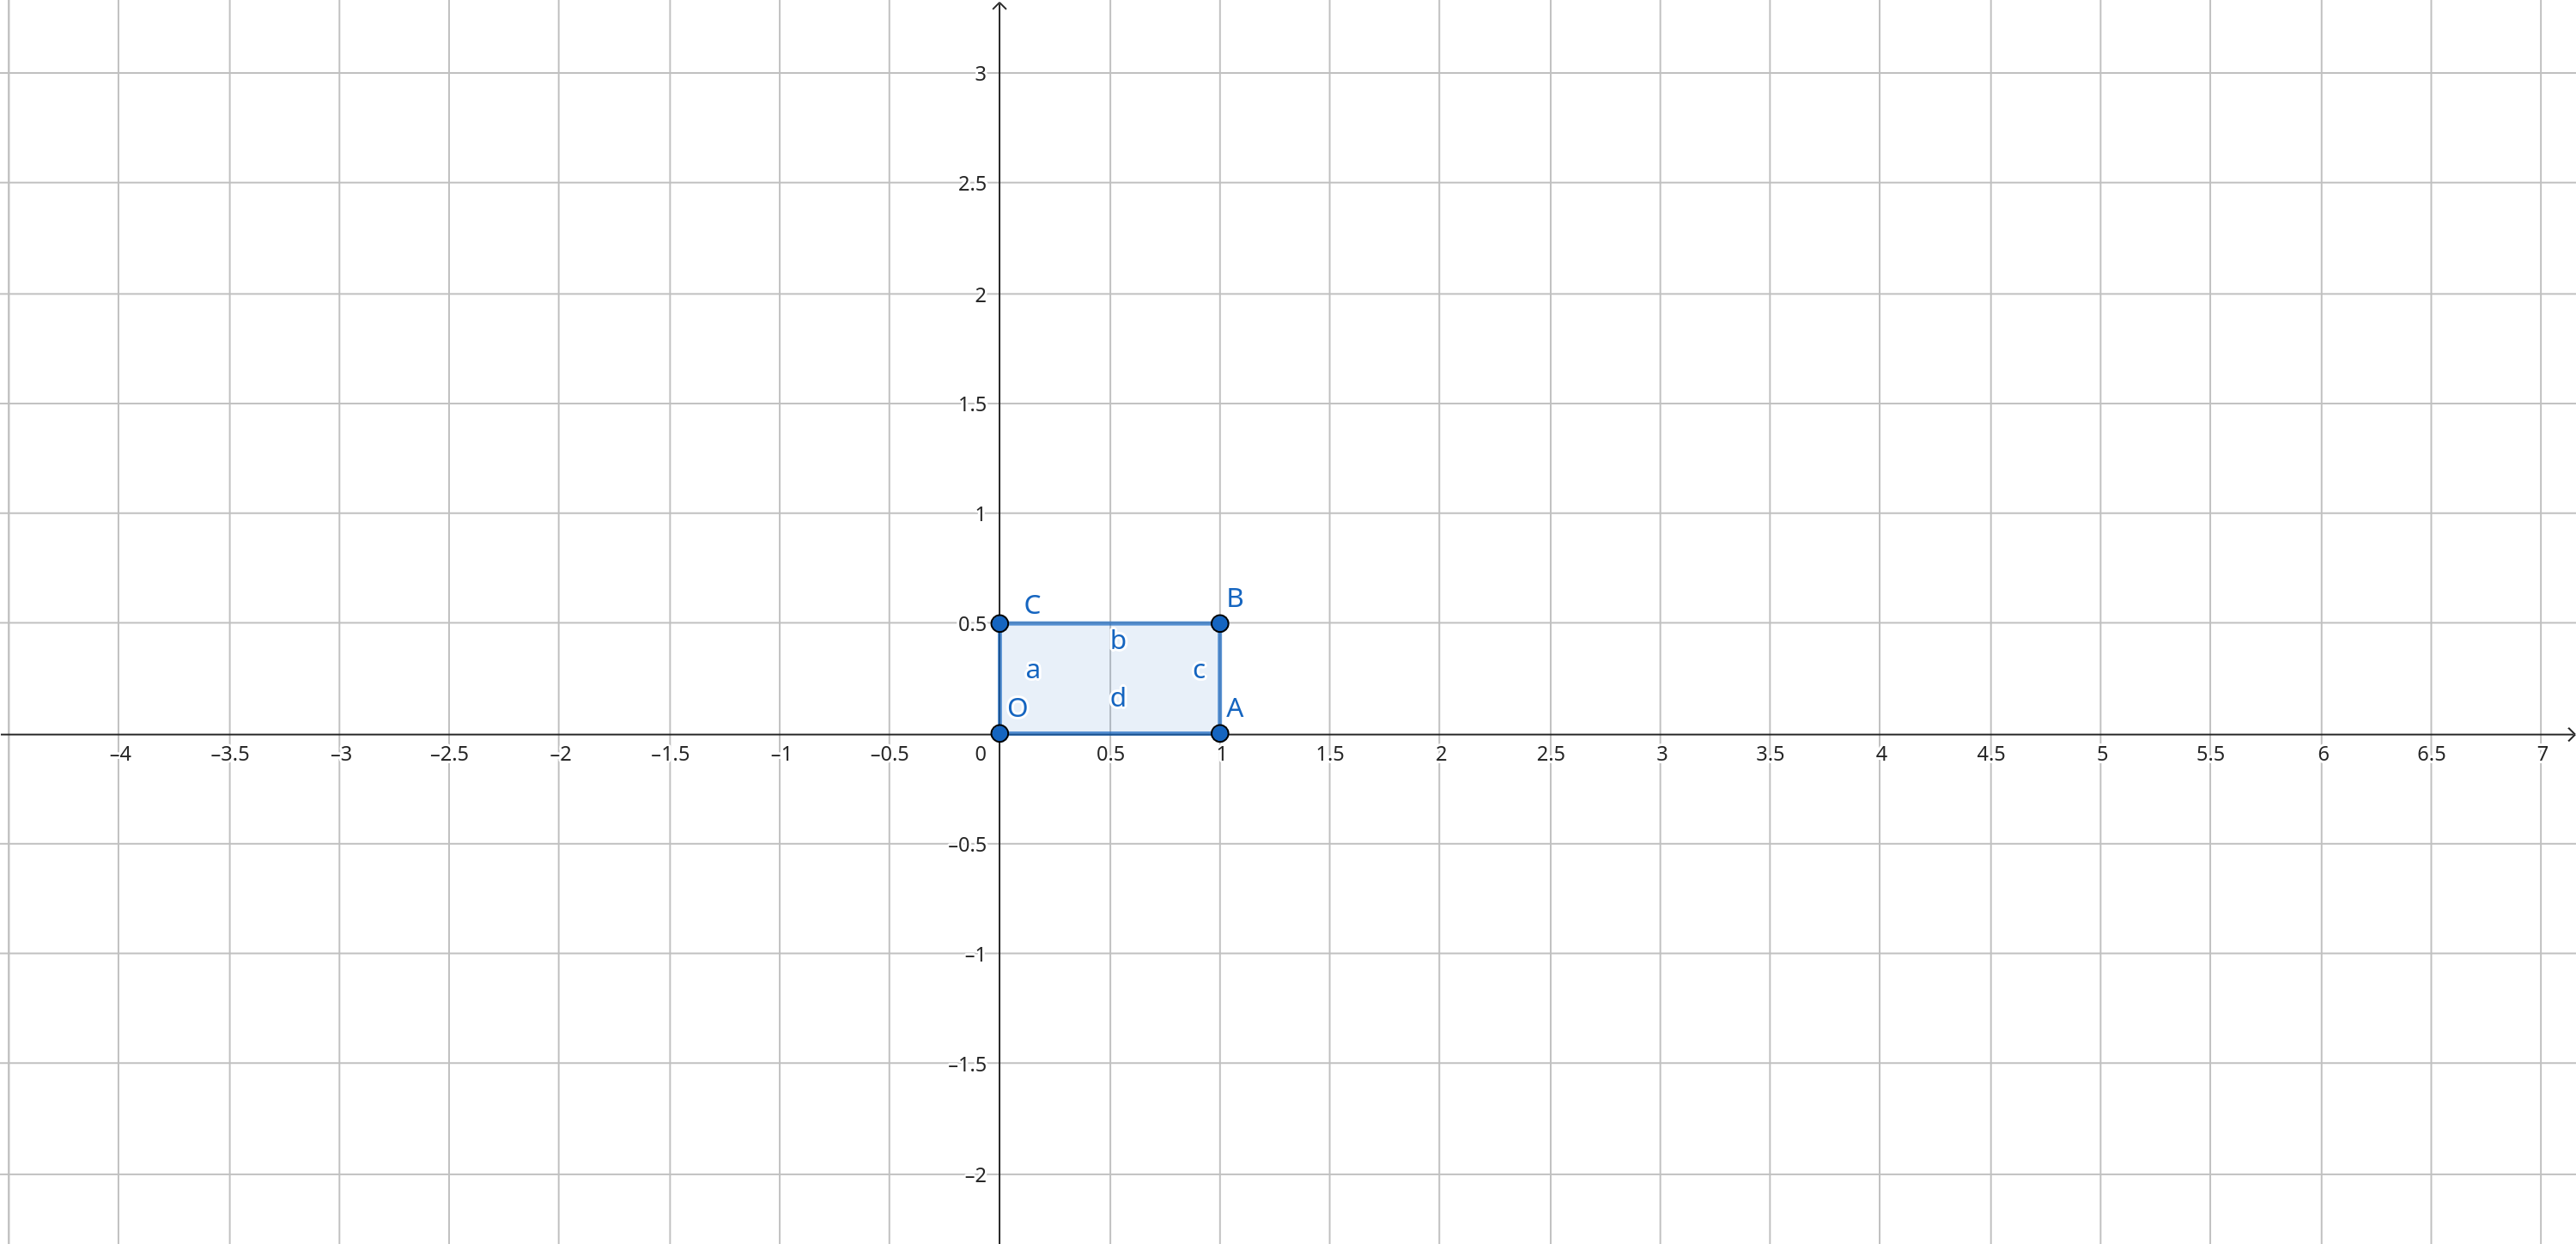
\includegraphics[width=0.75\linewidth]{geogebra-export(9).png}

    (i)

    $C = (k, 1)^T, \ B = (k + 1, 1)^T$
    
        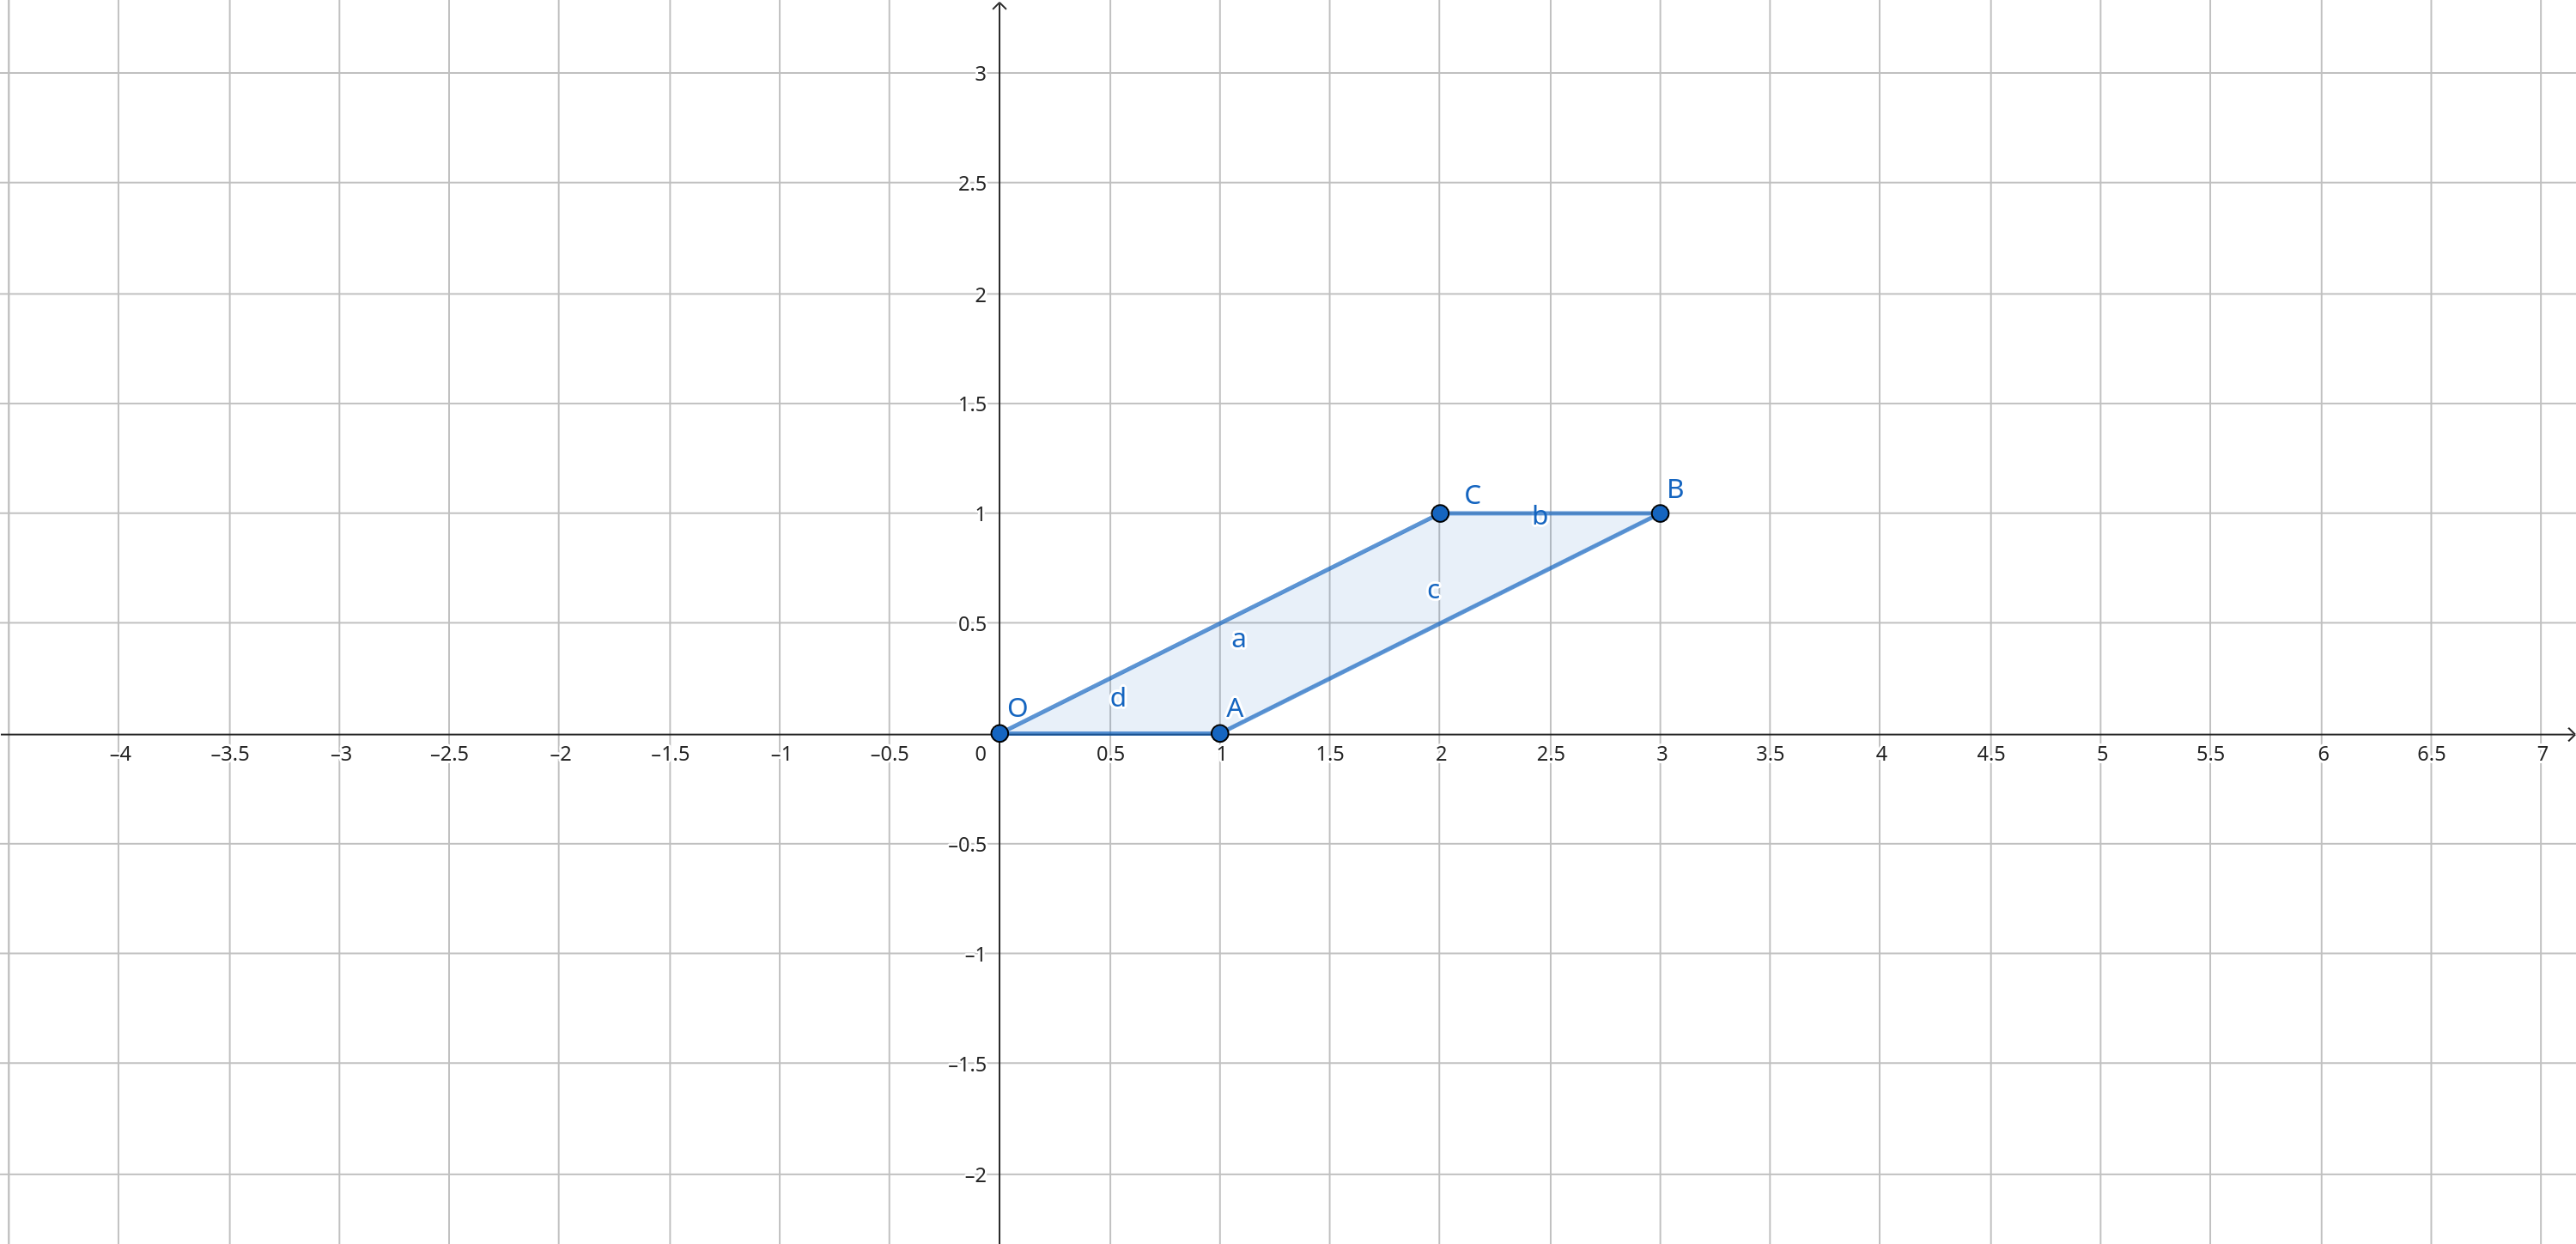
\includegraphics[width=0.75\linewidth]{geogebra-export(10).png}

            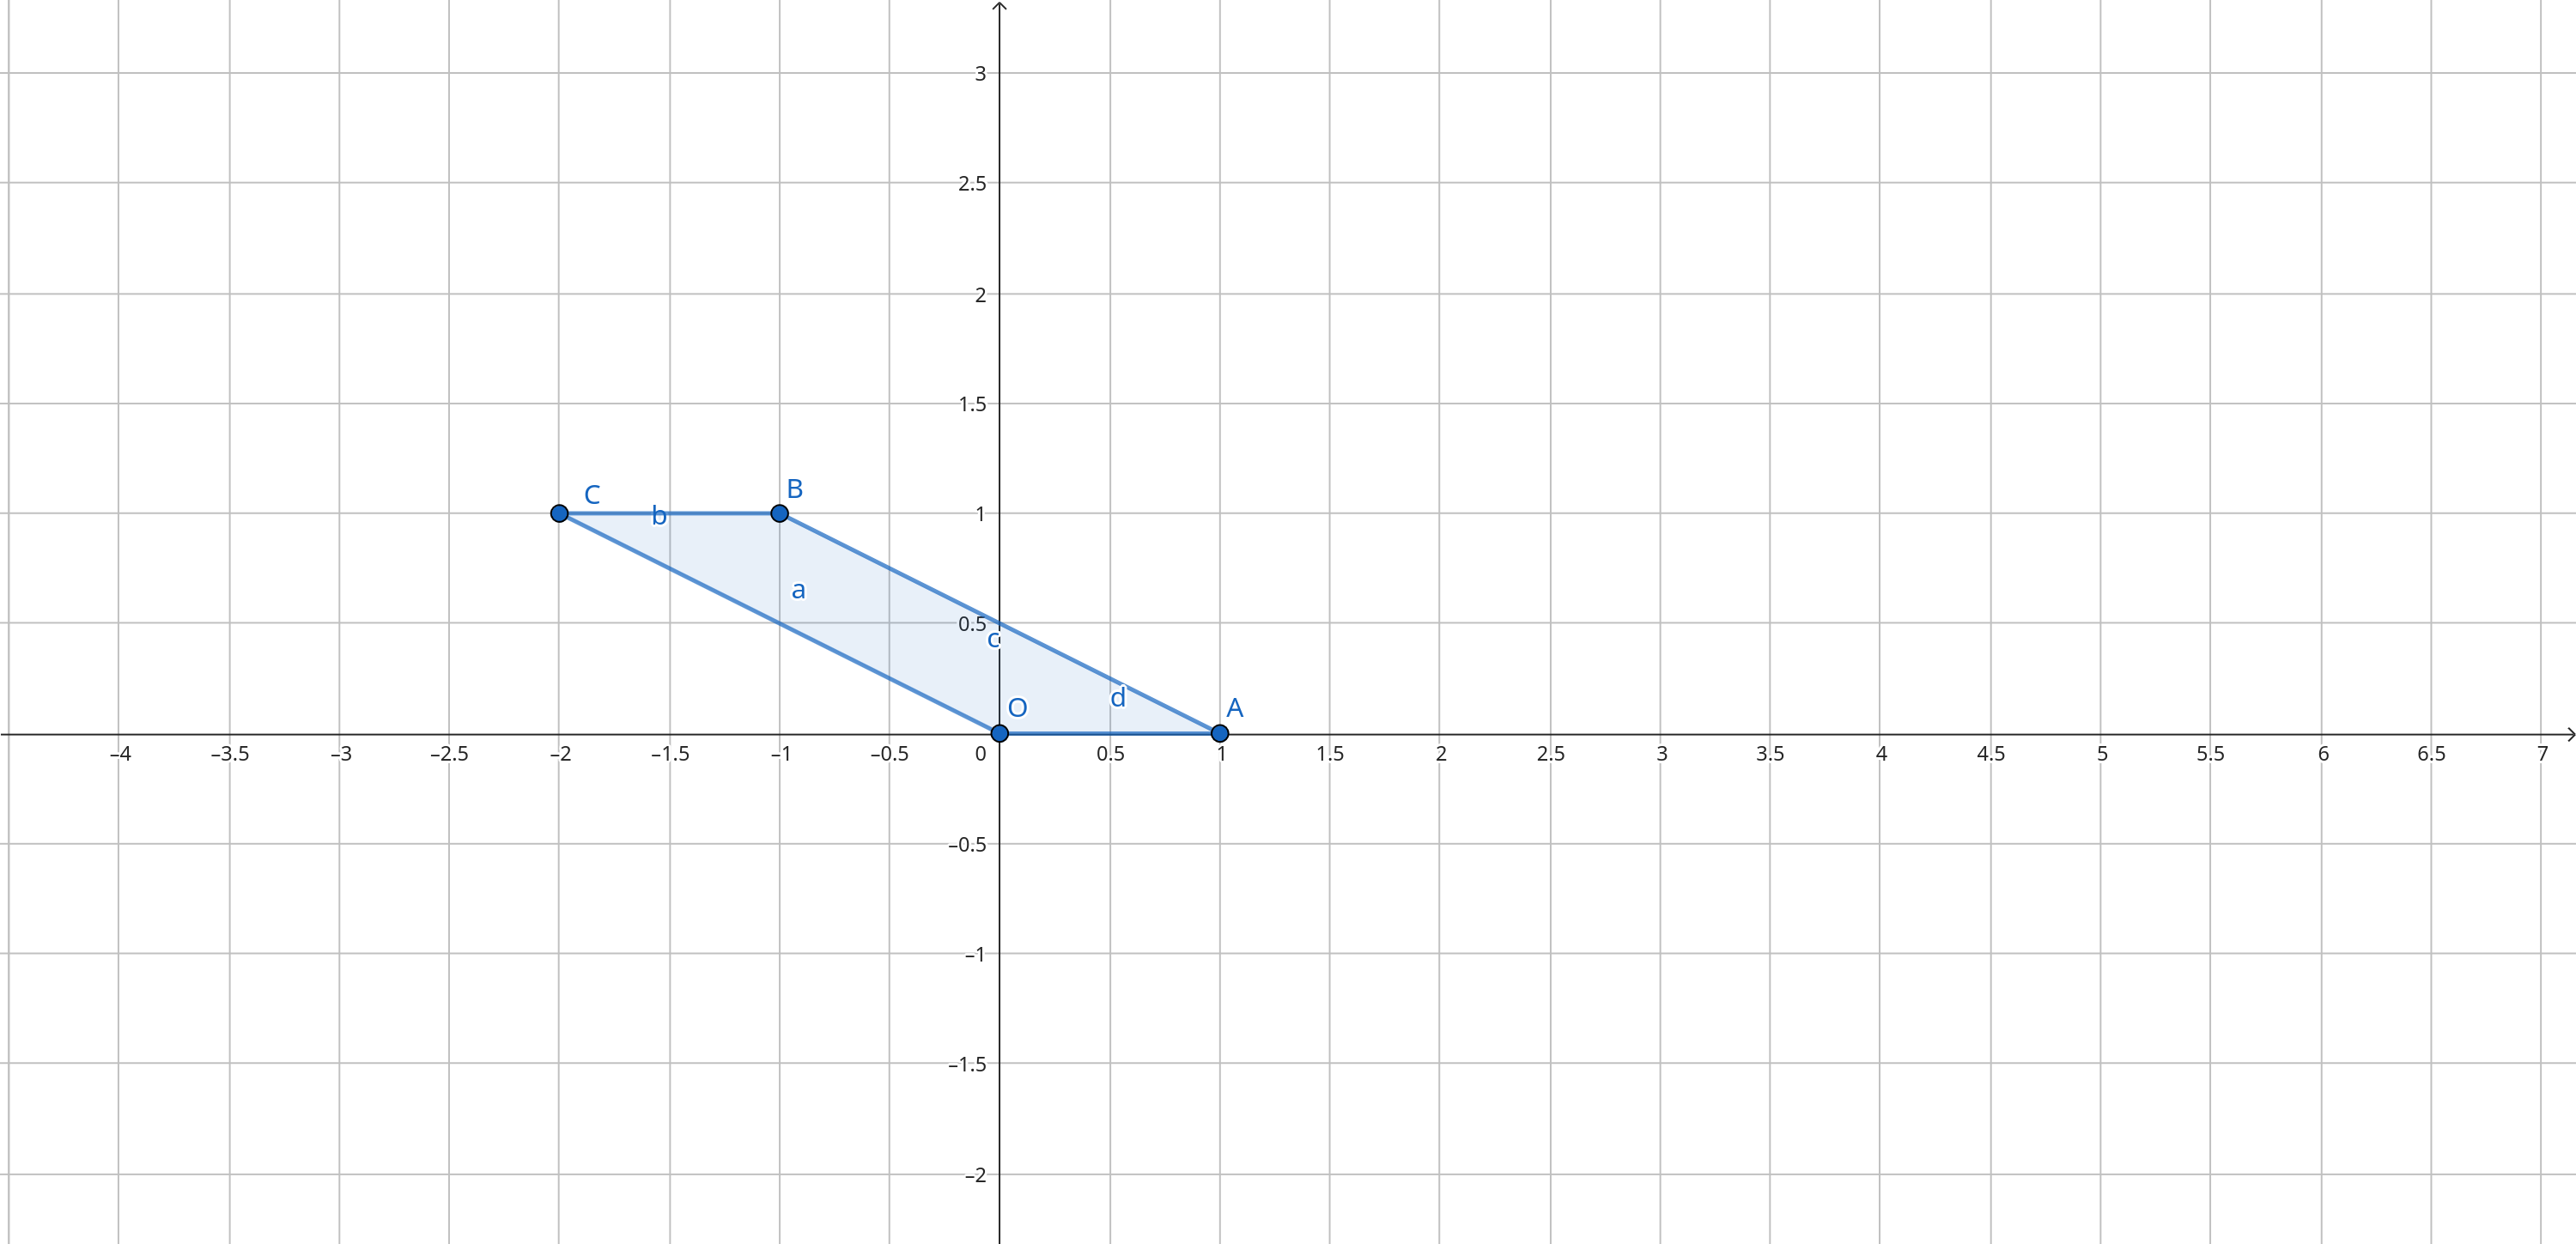
\includegraphics[width=0.75\linewidth]{geogebra-export(11).png}

    (j)

    $A = (1, k)^T, \ B = (1, k + 1)^T$
    
        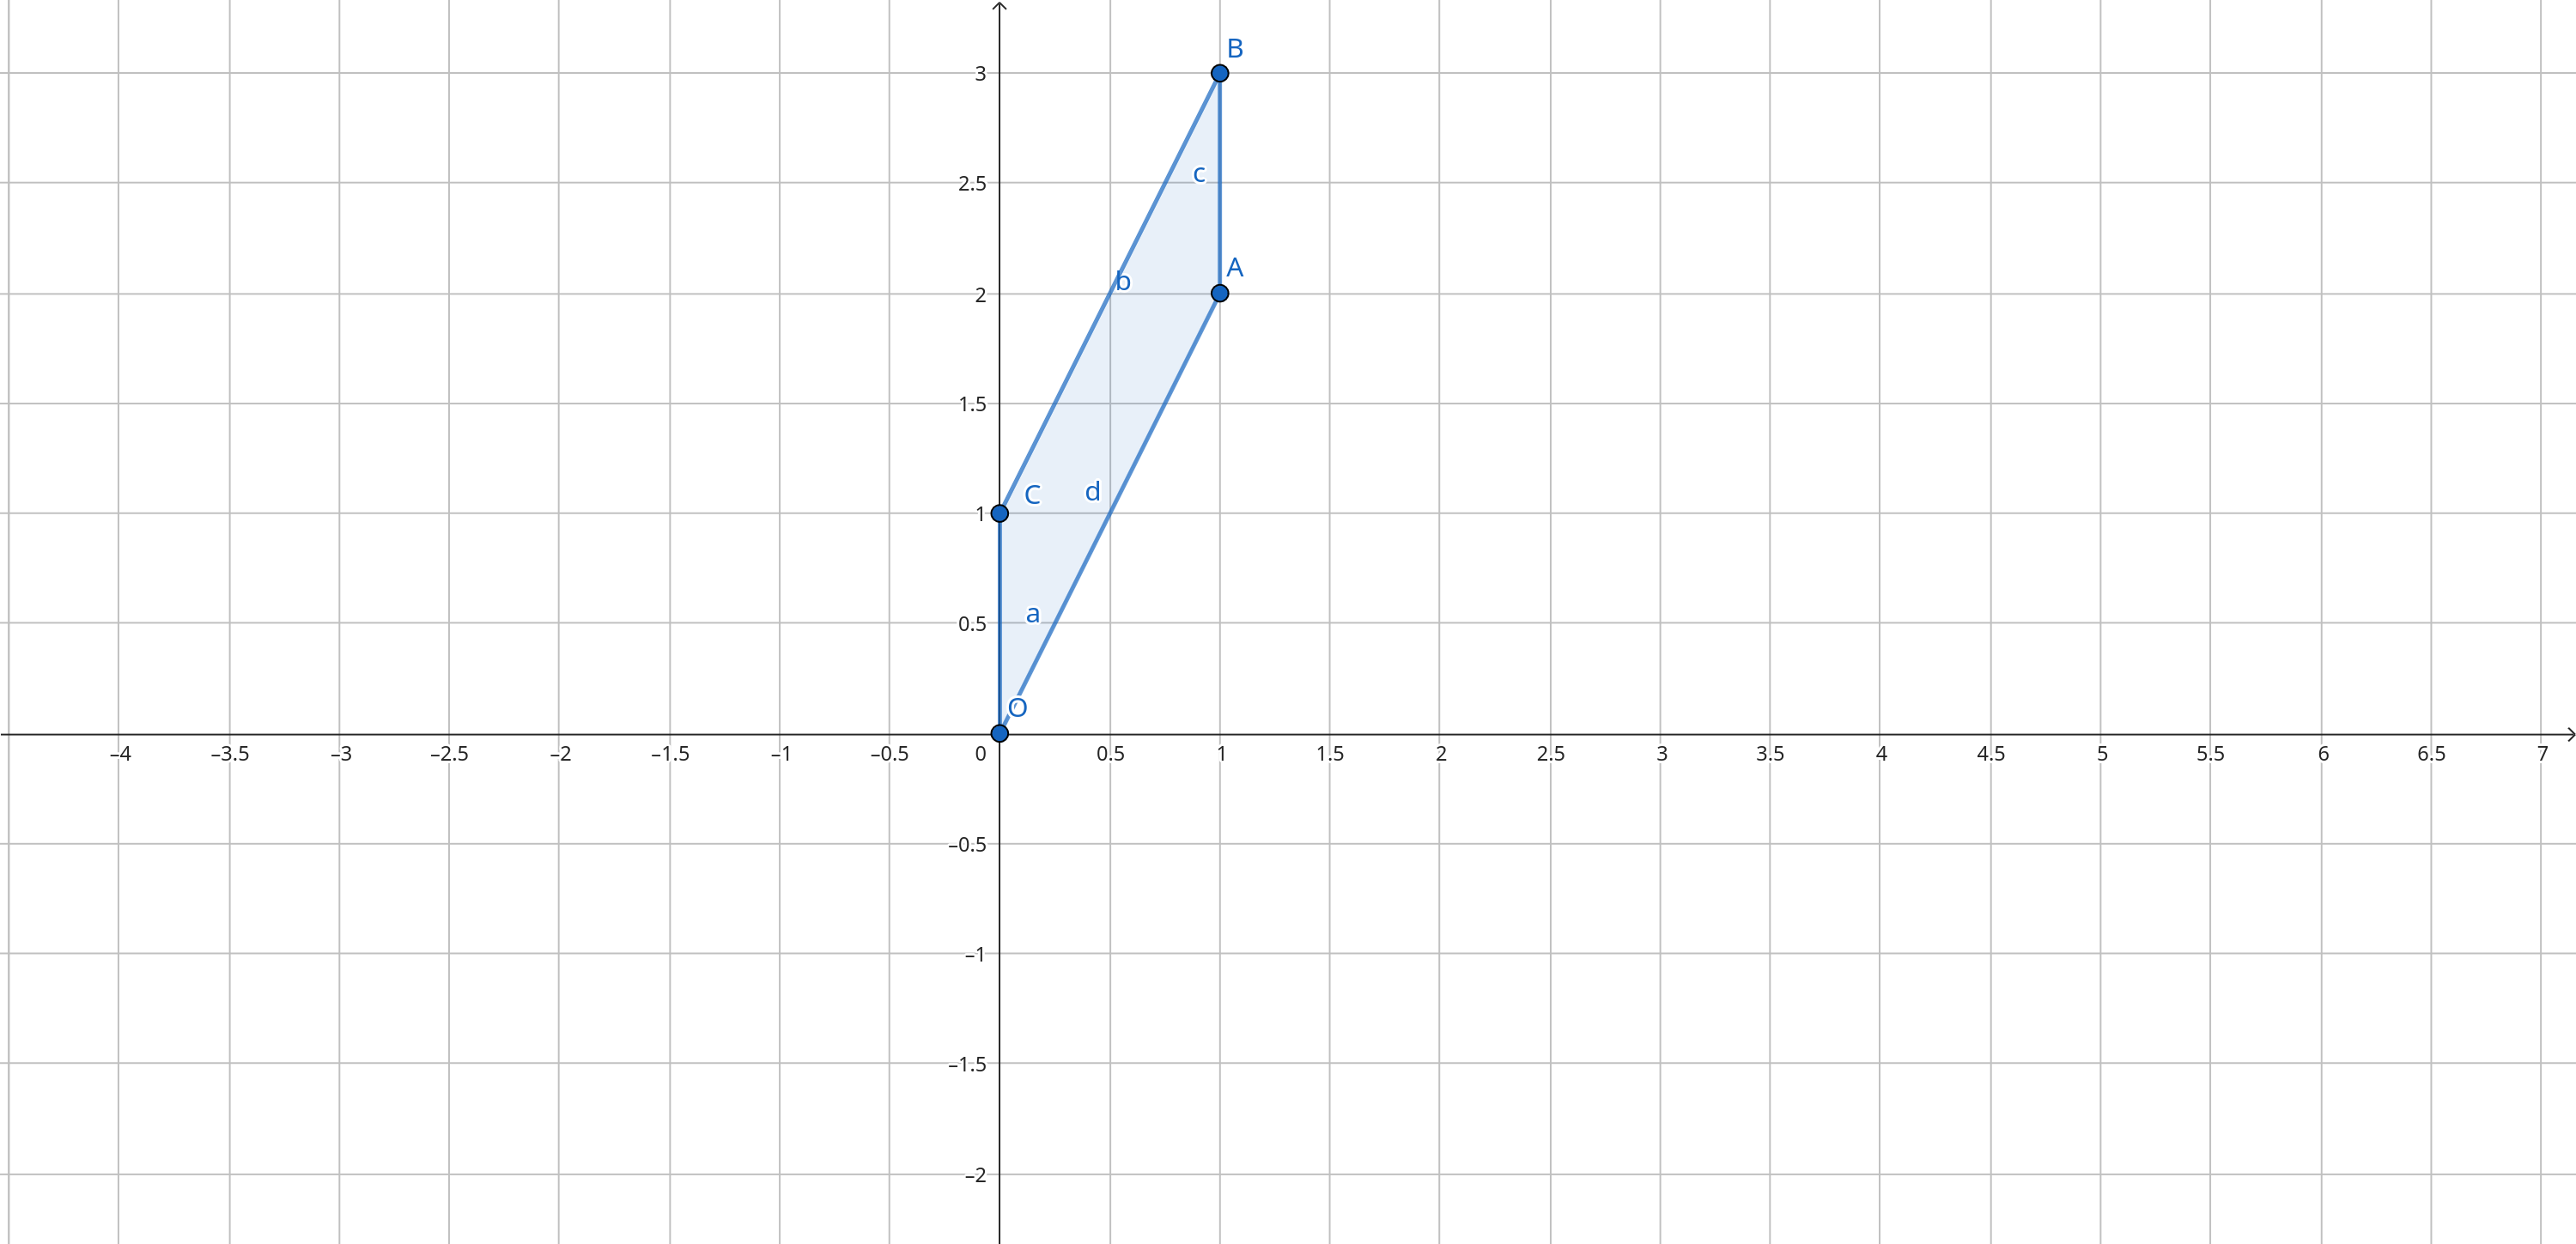
\includegraphics[width=0.75\linewidth]{geogebra-export(12).png}

        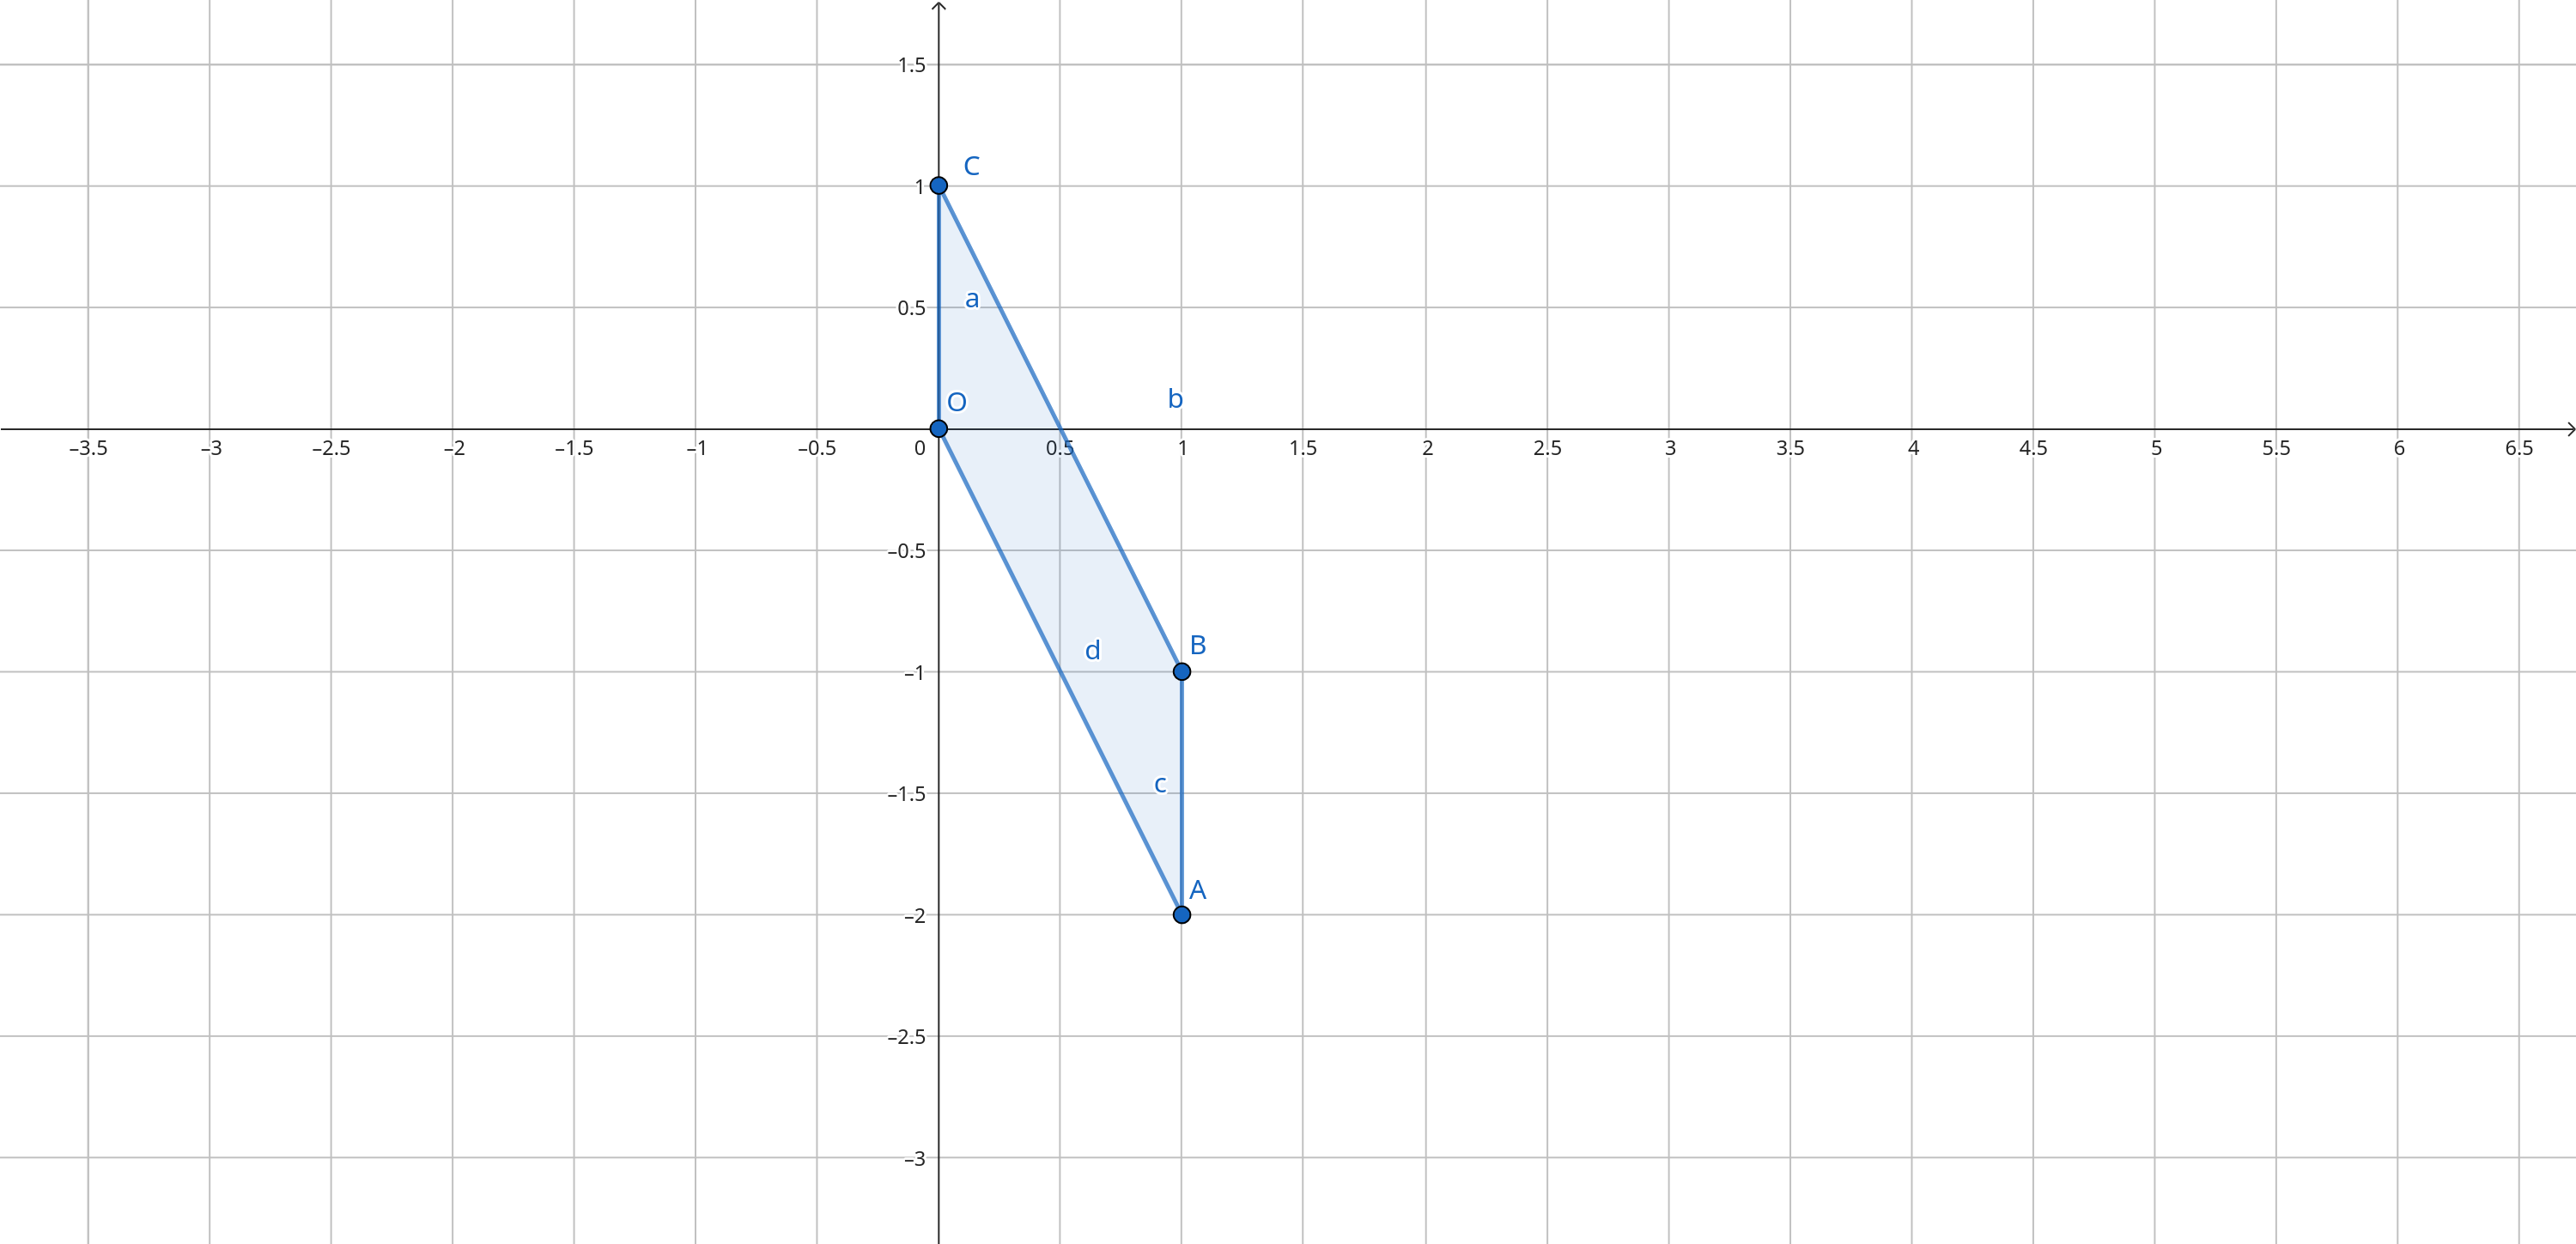
\includegraphics[width=0.75\linewidth]{geogebra-export(15).png}

    (k) 
    
            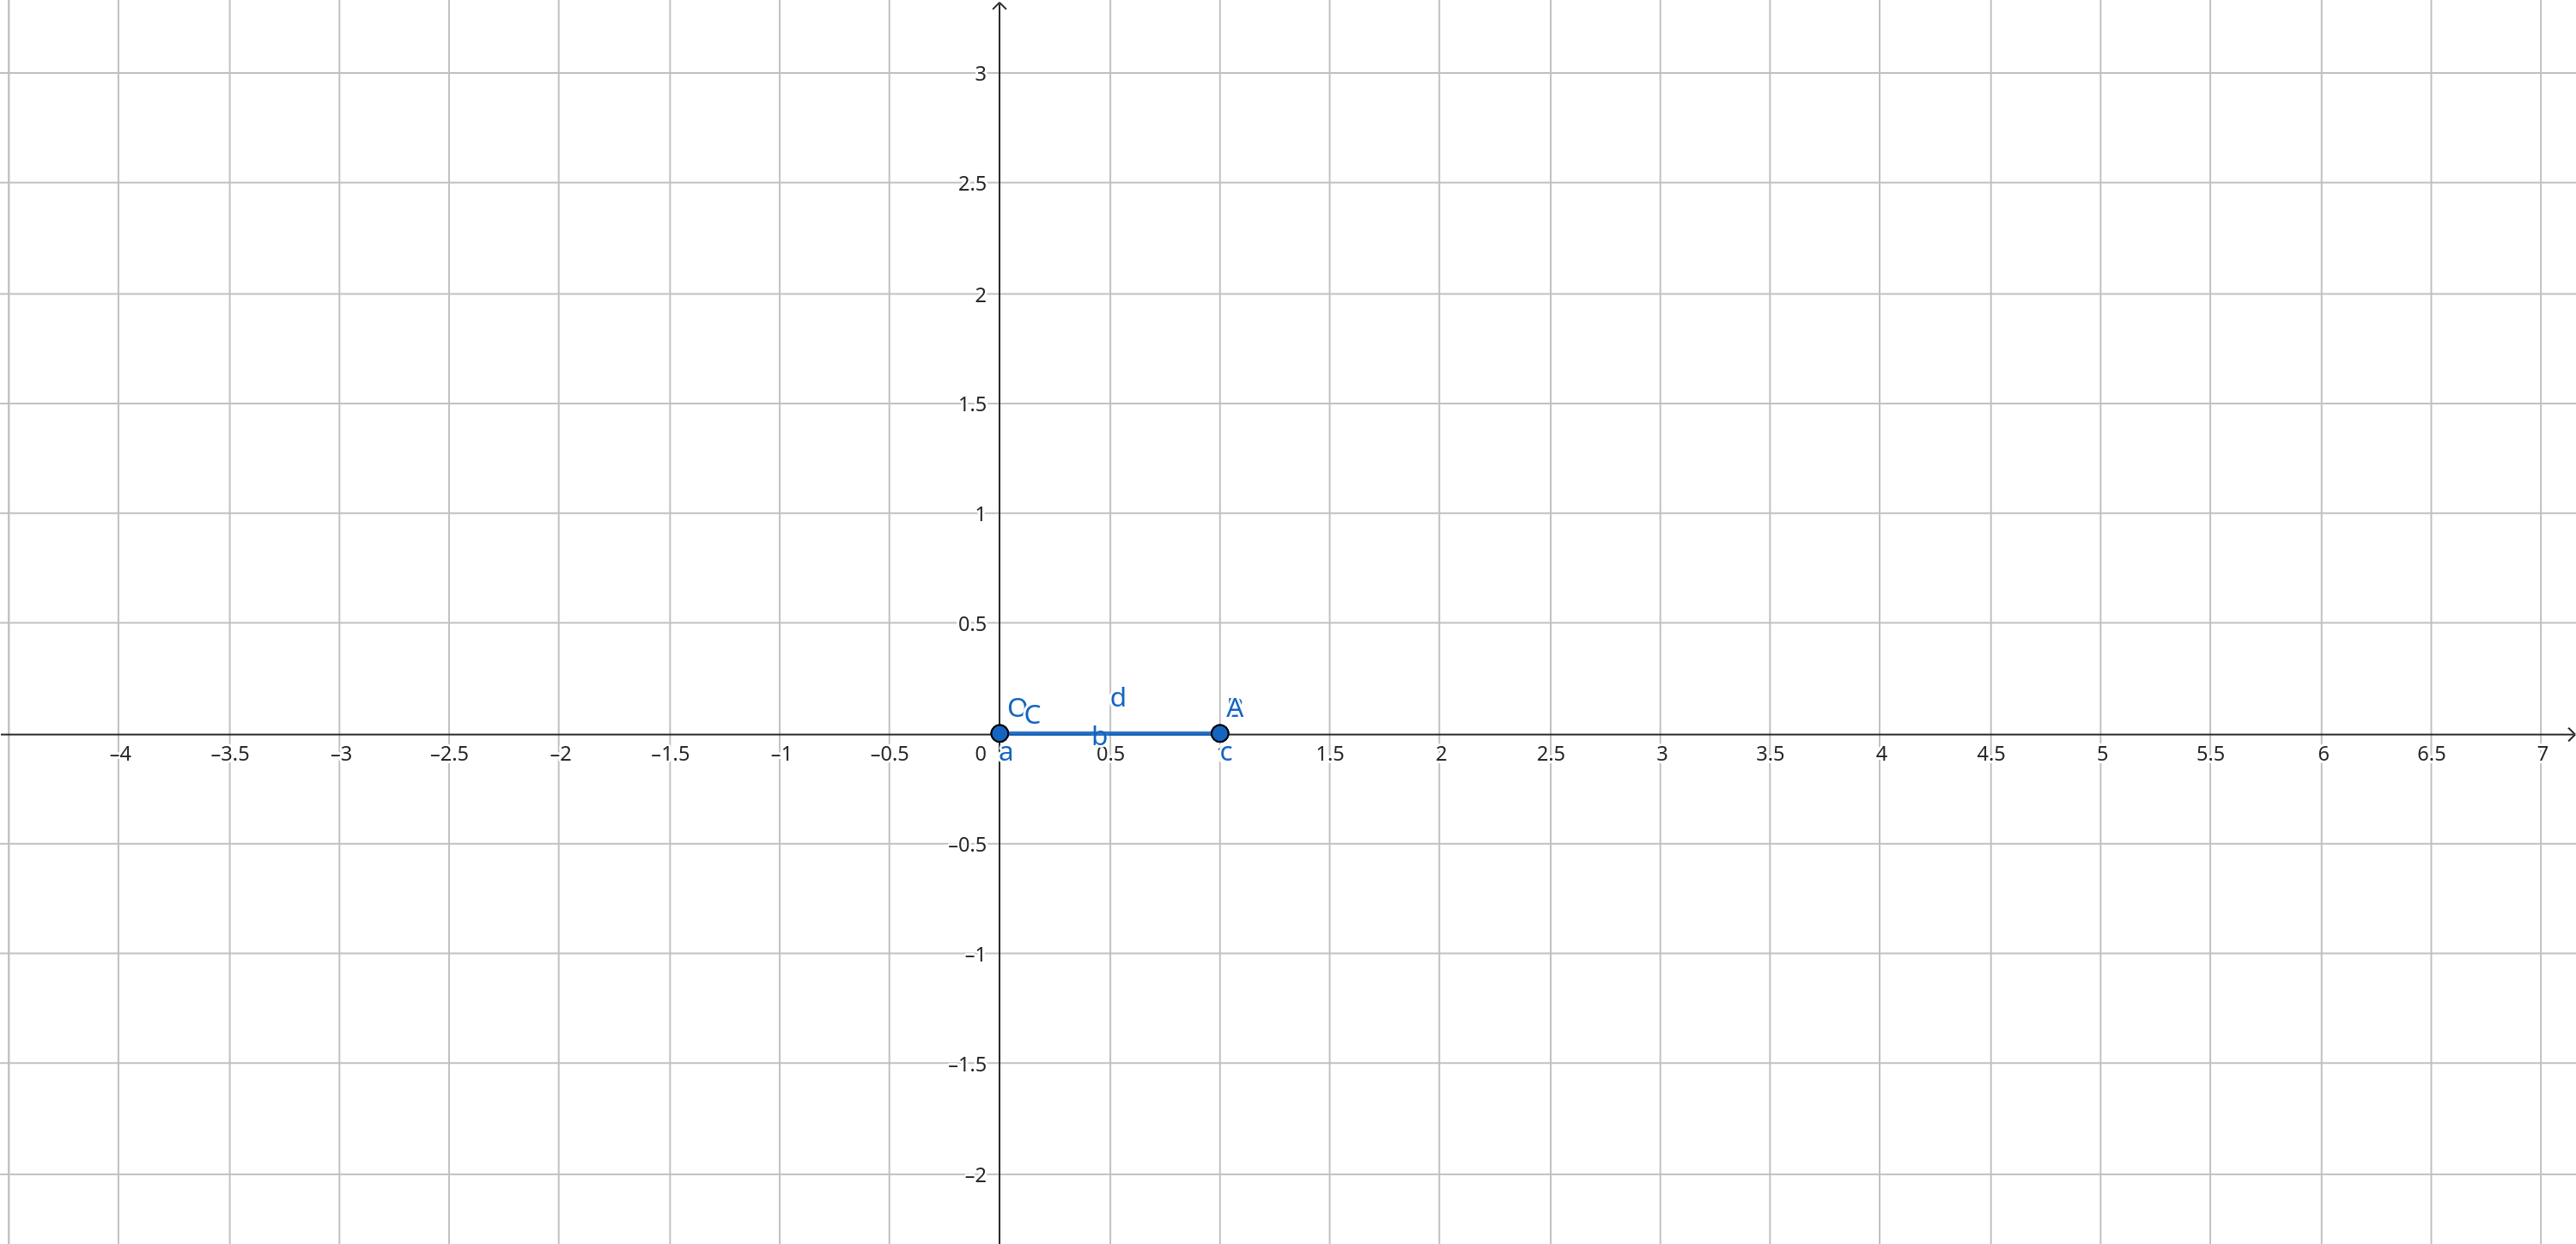
\includegraphics[width=0.75\linewidth]{geogebra-export(13).png}

    (l)

        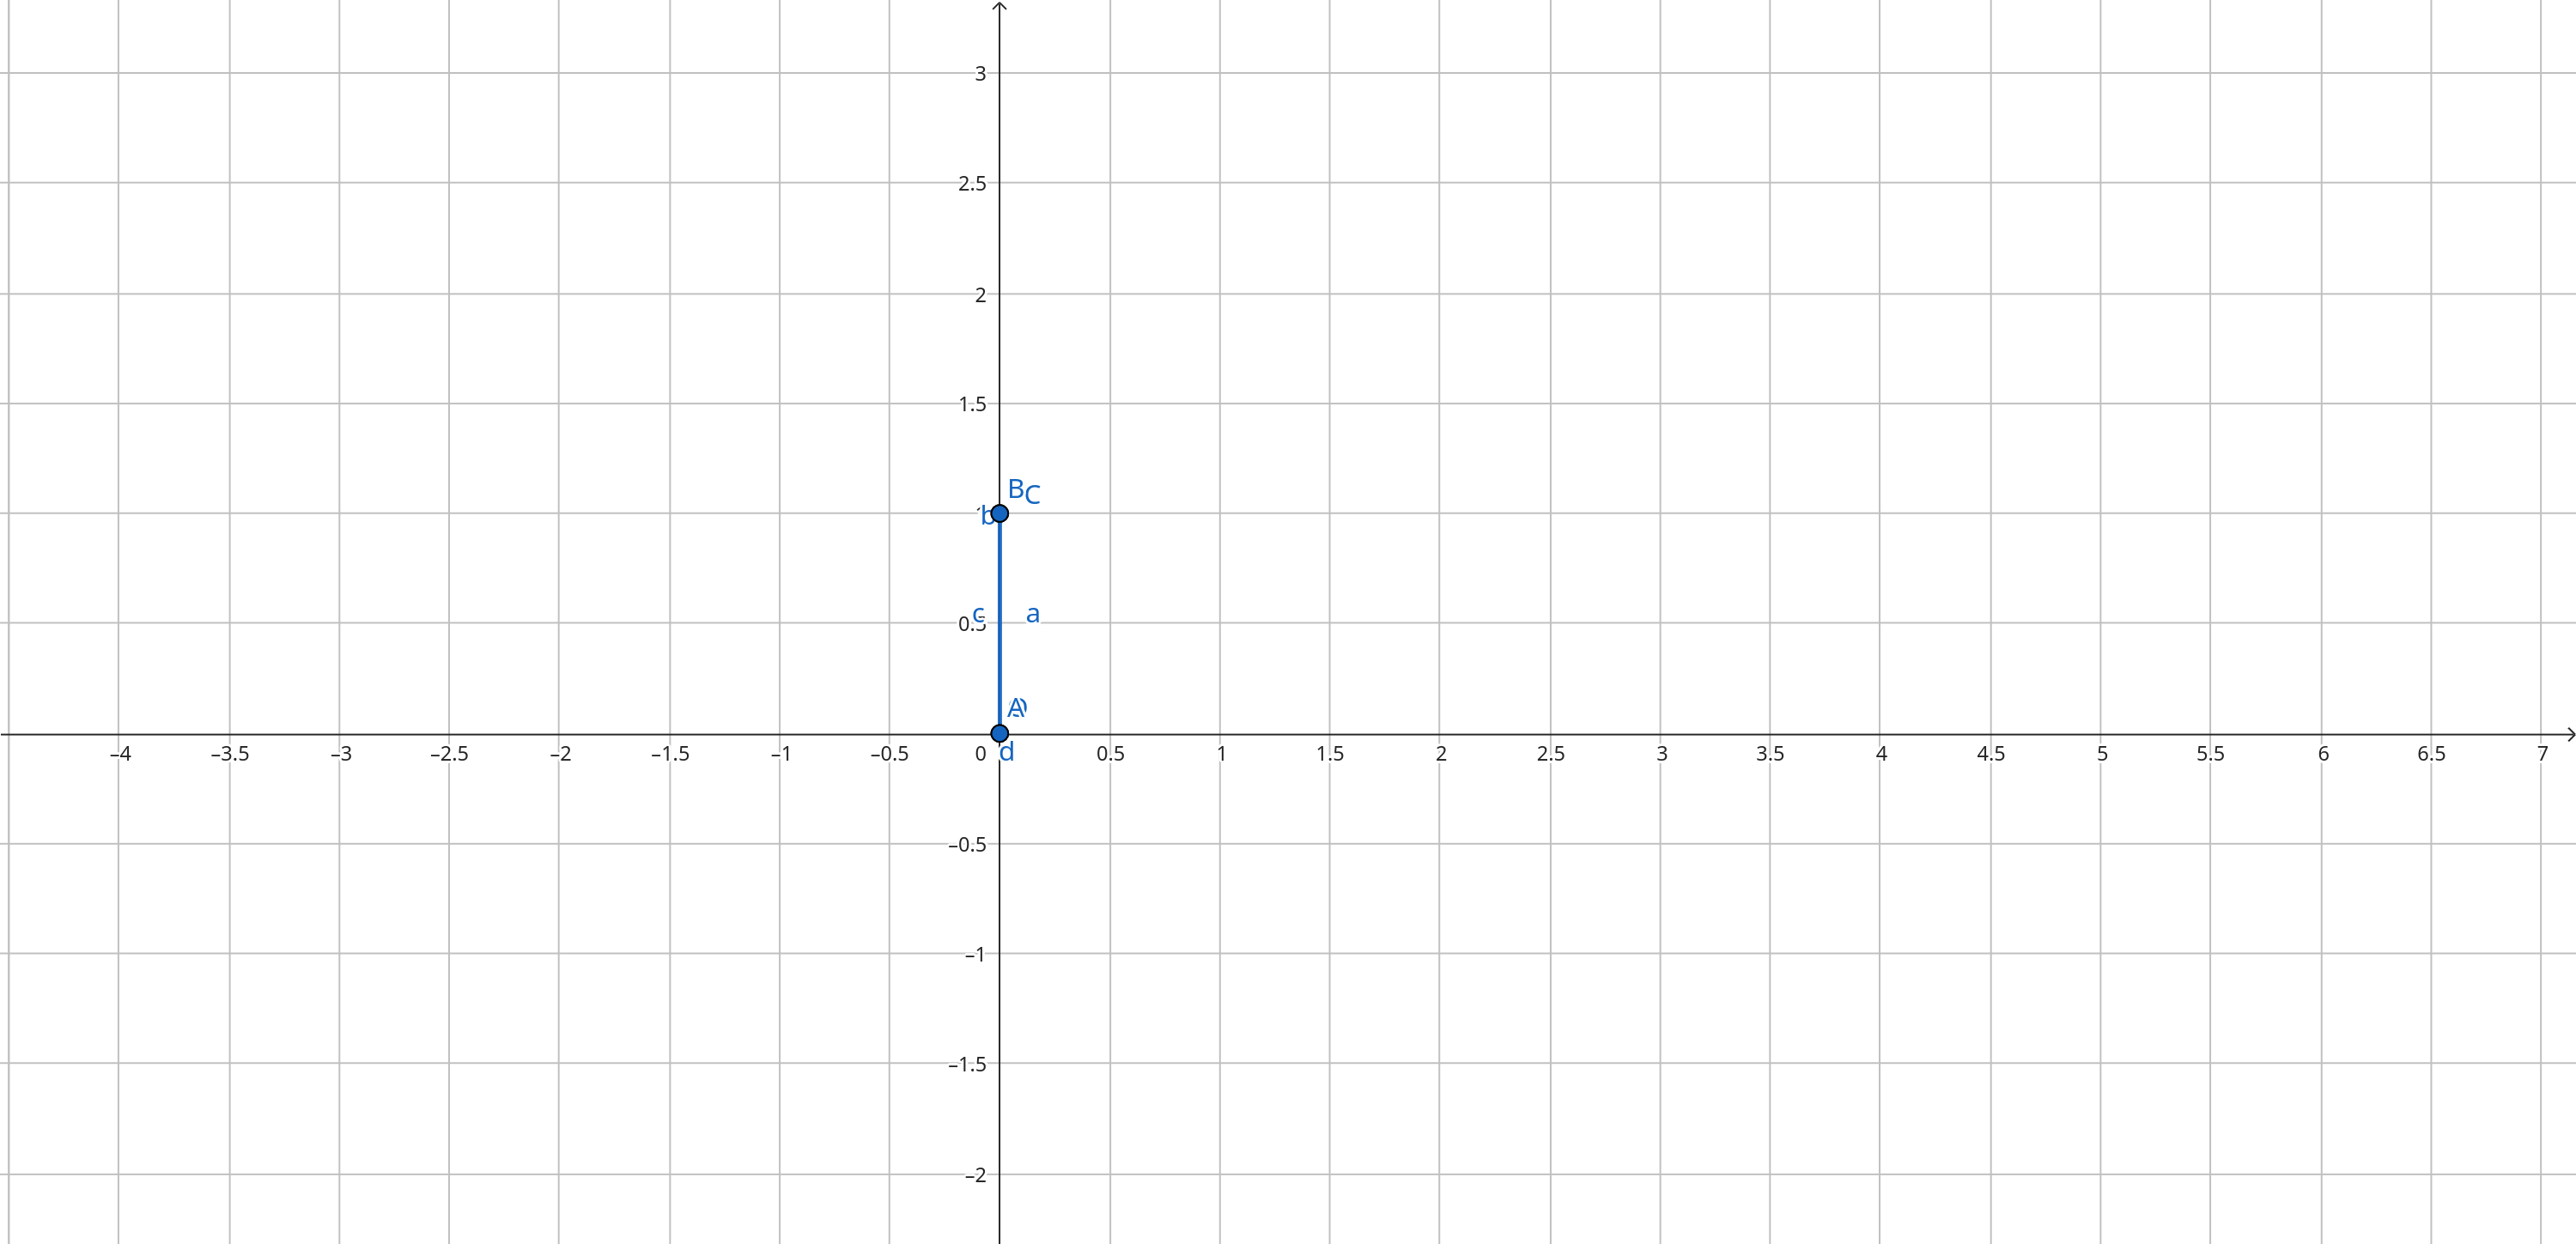
\includegraphics[width=0.75\linewidth]{geogebra-export(14).png}
\end{quote}

\textbf{\textsf{(3)}}
\begin{quote}
   \begin{itemize}
       \item $\varphi_1 = \begin{pmatrix} 0  & 0 & 0 & 0 \\ 1 & 1 & 0 & 0 \\ 0 & 1 & 1 & 0 \\ 0 & 0 & 1 & 1\end{pmatrix} \quad n = m = 4$

       \item $\varphi_2 = \begin{pmatrix} -3  & 2  \\ 1 & -4\\  0 & 0 \\  0 & 1\end{pmatrix} \quad n = 2, \ m = 4$

       
       \item $\varphi_3 = \begin{pmatrix} 1 & -5 & 4 \\ 0 & 1 & -6 \end{pmatrix} \quad n = 3, \ m = 2$
       
       \item $\varphi_4 = \begin{pmatrix} 2 & 0 & 3 & -4 \end{pmatrix} \quad n = 4, \ m = 1$
   \end{itemize} 
\end{quote}

\textbf{\textsf{(4)}}
\begin{quote}

Надем матрицу преобразования $A_{\varphi}$:

$
\begin{cases}
    \begin{pmatrix}
        a & b \\ c & d \\ f & e
    \end{pmatrix} \cdot \begin{pmatrix}1 \\ 2\end{pmatrix} = \begin{pmatrix} -3 \\ 5 \\ -1\end{pmatrix} \\
    \begin{pmatrix}
        a & b \\ c & d \\ f & e
    \end{pmatrix} \cdot \begin{pmatrix}-1 \\ 1\end{pmatrix} = \begin{pmatrix} -3 \\ 4 \\ -5\end{pmatrix}
\end{cases} \Longleftrightarrow$
$
\begin{cases}
    a + 2b = -3 \\
    c + 2d = 5 \\
    f + 2e = -1 \\
    -a + b = -3 \\
    -c + d = 4 \\
    -f + e = -5
\end{cases}
$

$
\begin{pmatrix}
1 & 2 & 0 & 0 & 0 & 0 & | & -3 \\    
0 & 0 & 1 & 2 & 0 & 0 & | & 5 \\    
0 & 0 & 0 & 0 & 1 & 2 & | & -1 \\    
-1 & 1 & 0 & 0 & 0 & 0 & | & -3 \\    
0 & 0 & -1 & 1 & 0 & 0 & | & 4 \\    
0 & 0 & 0 & 0 & -1 & 1 & | & -5 \\    
\end{pmatrix} \overset{r_4 += r_1, \ r_5 += r_2, \ r_6 += r_3}{\sim}
\begin{pmatrix}
1 & 2 & 0 & 0 & 0 & 0 & | & -3 \\    
0 & 0 & 1 & 2 & 0 & 0 & | & 5 \\    
0 & 0 & 0 & 0 & 1 & 2 & | & -1 \\    
0 & 3 & 0 & 0 & 0 & 0 & | & -6 \\    
0 & 0 & 0 & 3 & 0 & 0 & | & 9 \\    
0 & 0 & 0 & 0 & 0 & 3 & | & -6 \\    
\end{pmatrix} \sim
\begin{pmatrix}
1 & 2 & 0 & 0 & 0 & 0 & | & -3 \\    
0 & 0 & 1 & 2 & 0 & 0 & | & 5 \\    
0 & 0 & 0 & 0 & 1 & 2 & | & -1 \\    
0 & 1 & 0 & 0 & 0 & 0 & | & -2 \\    
0 & 0 & 0 & 1 & 0 & 0 & | & 3 \\    
0 & 0 & 0 & 0 & 0 & 1 & | & -2 \\    
\end{pmatrix} \overset{r_1 += -2r_4, \ r_2 += -2r_5, \ r_3 += -2r_6}{\sim}
\begin{pmatrix}
1 & 0 & 0 & 0 & 0 & 0 & | & 1 \\    
0 & 0 & 1 & 0 & 0 & 0 & | & -1 \\    
0 & 0 & 0 & 0 & 1 & 0 & | & 3 \\    
0 & 1 & 0 & 0 & 0 & 0 & | & -2 \\    
0 & 0 & 0 & 1 & 0 & 0 & | & 3 \\    
0 & 0 & 0 & 0 & 0 & 1 & | & -2 \\    
\end{pmatrix}
$

Получается, 
$A_{\varphi} = \begin{pmatrix}
   1 & - 2 \\ -1 & 3 \\ 3 & - 2 
\end{pmatrix}$

$A_{\varphi} \cdot \textbf{v} = (-1, \ 4, \ 9)^T, \ \textbf{v} = (x, \ y)^T \Longleftrightarrow 
\begin{cases}
x - 2y = -1 \quad (1)\\
-x + 3y = 4 \quad (2)\\
3x -2y = 9 \quad (3)
\end{cases}
$ 

$(1) + (2): \ y = 3$, подставим в $(3)$: $3x - 2 \cdot 3 = 9 \Leftrightarrow x = 5$

$\textbf{v} = (5, \ 3)^T$

\boxed{\text{Ответ: $(5, \ 3)^T$}}
\end{quote}

\end{document}